\documentclass{article}

\usepackage{arxiv}

\usepackage[utf8]{inputenc}
\usepackage[T1]{fontenc}
\usepackage{hyperref}
\usepackage{url}
\usepackage{booktabs}
\usepackage{amsmath, amssymb, amsthm}
\usepackage{amsfonts}
\usepackage{bm}
\usepackage{nicefrac}
\usepackage{microtype}
\usepackage{graphicx}
\usepackage{subcaption}
\usepackage{xcolor}
\usepackage[numbers,sort&compress]{natbib}

%%% see my comments with the '%%%' notation


\newcommand{\synfig}[1]{notebooks/figures/synthetic/gene_expression_synthetic/imaging_synthetic/#1}
\newcommand{\simfig}[1]{notebooks/figures/synthetic/#1}
\newcommand{\sumfig}[1]{notebooks/figures/#1}
\newcommand{\kircfig}[1]{notebooks/figures/tcga_kirc/gene_expression/organ_radiomics/#1}
\newcommand{\wsifig}[1]{notebooks/figures/tcga_kirc/gene_expression/wsi/#1}
\newcommand{\wsiNslides}{580}
\newcommand{\wsiNcases}{190}
\newcommand{\wsiNfeat}{54}
\newcommand{\wsiRone}{0.46}
\newcommand{\wsiN}{189}
\newcommand{\wsiRoneCT}{0.11}
\newcommand{\wsiNCT}{190}
\newcommand{\wsiRank}{3}
\newcommand{\wsiPmax}{0.003}
\newcommand{\wsiMI}{2.2}
\newcommand{\wsiMICT}{1.6}
\newcommand{\wsiRoneNormal}{0.02}
\newcommand{\wsiNnormal}{167}
\newcommand{\wsiRoneTumorM}{0.39}
\newcommand{\wsiRoneNormalM}{0.02}
\newcommand{\wsiNmatched}{167}
\newcommand{\wsiDecRaw}{0.45}
\newcommand{\wsiDecDecon}{0.49}

\newcommand{\nsclcfig}[1]{notebooks/figures/nsclc/gene_expression/organ_radiomics_subset/#1}
\newcommand{\adnifig}[1]{notebooks/figures/adni/gene_expression/fastsurfer/#1}

\newtheorem{proposition}{Proposition}
\newtheorem{definition}{Definition}
\newtheorem{corollary}{Corollary}

\newcommand{\R}{\mathbb{R}}
\newcommand{\E}{\mathbb{E}}
\newcommand{\N}{\mathcal{N}}
\newcommand{\Cov}{\operatorname{Cov}}
\newcommand{\Var}{\operatorname{Var}}
\newcommand{\rank}{\operatorname{rank}}
\newcommand{\tr}{\operatorname{tr}}
\newcommand{\Sg}{\Sigma_{G}}
\newcommand{\Sx}{\Sigma_{X}}
\newcommand{\Sgx}{\Sigma_{GX}}
\newcommand{\Sxg}{\Sigma_{XG}}
\newcommand{\Sgcx}{\Sigma_{G\mid X}}
\newcommand{\T}{^{\top}}

\title{Image-Identifiable Genomic Subspaces:\\
A Linear--Gaussian Model of Radiogenomic Recoverability}

\author{
Joseph Rich$^{1,2}$ \and
Raphi Kang$^{1,3}$ \and
David Jin$^{1}$ \and
Pietro Perona$^{1,3}$ \and
Lior Pachter$^{1,3}$\thanks{Address correspondence to \texttt{lpachter@caltech.edu}.}
}

\date{
\small
$^1$ Division of Biology and Biological Engineering, California Institute of Technology\\
$^2$ Keck School of Medicine, University of Southern California\\
$^3$ Division of Computing and Mathematical Sciences, California Institute of Technology
}

\renewcommand{\shorttitle}{Image-Identifiable Genomic Subspaces}

\hypersetup{
pdftitle={Image-Identifiable Genomic Subspaces: A Linear-Gaussian Model of Radiogenomic Recoverability},
pdfauthor={Joseph Rich, Lior Pachter},
pdfkeywords={radiogenomics, canonical correlation analysis, mutual information, recoverability, linear-Gaussian model},
}

\begin{document}
\maketitle

\begin{abstract}
How much of a patient's genomic state can be read off their scan? We answer this
with a number, in bits, that a study of a given size cannot exceed. Starting
from a linear--Gaussian channel in which the genomic state $g\in\R^p$ is
Gaussian and the imaging phenotype $x\in\R^d$ is a noisy linear readout of it,
the classical theory gives the \emph{channel} information $I(g;x)$ and identifies
the maximally recoverable genomic directions with canonical correlation
analysis. That is an infinite-data quantity, and it is not what a cohort can
demonstrate. Our main contribution is the finite-sample counterpart: for any
learning algorithm trained on $n$ patients with a $d^\star$-dimensional imaging
representation, the attainable out-of-sample recoverability of a genomic
direction obeys
$\mathcal{R}_n = \rho^2\,n/(n+\nu)$ with $\nu = d^\star(1-\rho^2)/\rho^2$, giving
an \emph{attainable information} $\mathcal{I}_n =
-\tfrac12\sum_i\log(1-\mathcal{R}_{n,i})$ that is zero at $n=0$ and reaches
$I(g;x)$ only as $n\to\infty$. Two consequences are immediate: the learning cost
$\nu$ is simply the feature count divided by the channel signal-to-noise ratio,
and attainable signal scales as $\rho^4$ rather than $\rho^2$, so weak genomic
directions are doubly penalized and cannot be certified at realistic $n$. We
verify the bound in simulation --- six model families, from ridge to gradient
boosting to a neural network, approach it and none crosses it --- and then
report it for three cohorts using a model-free upper confidence limit obtained
by planting signal of known strength into permuted real data and sweeping the
planted rank. Bounding a single scalar spectral functional, the fourth moment
$\sum_i\rho_i^4$, and converting it by a concavity argument that is exact over
every spectrum, the limit applies to \emph{total} retention across all
directions rather than to the single best axis, and without any assumption on
the shape of the spectrum. At their actual sizes, TCGA-KIRC ($n=190$, CT), an
NSCLC cohort ($n=129$, CT), and ADNI ($n=702$, MRI) admit at most $0.76$,
$0.18$ and $1.20$ bits per patient about the transcriptome --- around one
perfectly measured binary biomarker apiece, with the NSCLC statistic in fact
falling below its own permutation null --- and
equivalently a ceiling of $\mathrm{AUC}\le 0.76$--$0.83$ on \emph{any}
classifier for \emph{any} binarized genomic feature, which is where the
published per-gene AUCs in this literature in fact sit. Stress-testing the
bound against every combination of training-set size, genomic feature set and
learning algorithm --- $360$ configurations across the three cohorts --- no
combination crosses it, while $59$ of $60$ remain non-zero, so the ceiling is
neither violated nor vacuous. Reaching $90\%$ of even
these channels would take $n\approx 10^3$. Finally, a chain-rule decomposition
against hand-specified anchor genes shows the recoverable subspace is not
spread across the transcriptome: in both tumor cohorts a four-gene panel of
lineage and hypoxia markers accounts for most of the attainable information. The
practical message for radiogenomics is that the useful target is a handful of
genes and a reportable bit-count, not a transcriptome-wide search.
\end{abstract}

\keywords{radiogenomics \and canonical correlation analysis \and mutual information \and recoverability \and linear--Gaussian model}

\section{Introduction}
\label{sec:intro}

Radiogenomics asks how much of a molecular state
is written into its image~\citep{rutman2009radiogenomics,gillies2016radiomics,lambin2017radiomics,bodalal2019radiogenomics}.
Clinically, useful applications include those where knowledge of a molecular state would change management, including some cancers and neurodegenerative diseases, but the cost or risk of sequencing is prohibitive. 
For instance, in clear cell renal cell carcinoma, CT descriptors of margin,
enhancement and intratumoral vascularity have been tied to \emph{VHL} and to the
chromatin-modifying genes that co-occur with
it~\citep{karlo2014ccrcc,jamshidi2015ccrcc,shinagare2015ccrcc,udayakumar2024radiogenomic}.
In diffuse glioma, MR appearance carries \emph{IDH1} status and 1p/19q
codeletion well enough to support classifiers built on imaging
alone~\citep{zhou2017lgg,kickingereder2016gbm}. In lung adenocarcinoma, CT
phenotypes have been used to call \emph{EGFR} mutation
status~\citep{gevaert2012nsclc,bakr2018nsclcradiogenomics,wang2019egfr}.

None of these mappings is a lookup table from a single imaging sign to a single
variant. Whatever molecular state reaches the image reaches it diffusely,
through texture, shape, and spatial heterogeneity, so the field moved quickly
from hand-specified radiomic descriptors~\citep{lambin2012radiomics,aerts2014radiomics,vangriethuysen2017pyradiomics}
to representations learned from the images themselves~\citep{hosny2018ai,bi2019ai}.
Convolutional networks with residual connections~\citep{he2016resnet} are
trained end to end on volumes, and one such network classifies \emph{IDH1},
1p/19q and MGMT status directly from MRI~\citep{chang2018glioma}, as another
does for \emph{EGFR} from CT~\citep{wang2019egfr}. Encoder--decoder segmentation
networks supply the region of interest and increasingly the features as
well~\citep{ronneberger2015unet,isensee2021nnunet}; vision
transformers~\citep{dosovitskiy2021vit} model context across a whole volume
rather than a local receptive field; attention-based multiple-instance pooling
aggregates slices or patches into one patient-level
prediction~\citep{ilse2018abmil}; and large pretrained encoders are now used as
general-purpose imaging feature extractors~\citep{mei2022radimagenet,moor2023foundation}.

What almost none of this work asks is how much there was to find. The standard
output is a classifier and an AUC, and the usual reading is asymmetric: a weak
result is blamed on the model, a strong one is credited to biology. At the
cohort sizes typical of the field ($n\sim 10^2$) against panels of
$10^3$--$10^4$ transcripts, that reading is unsafe in both directions. This is a
high-dimensional, low-power multiple-testing problem in which apparent positives
are easily manufactured by overfitting, batch structure, or demographic
confounding~\citep{chalkidou2015fdr,welch2019vulnerabilities}. Absent a ceiling
there is no way to say whether an AUC of $0.7$ is near the limit of what the
scan encodes or a tenth of it, whether the next gain should come from more
patients or a better architecture, or when a search has been exhausted. We argue
that the more answerable question is not ``does imaging predict gene $j$?'' but
\emph{how many genomic directions are image-identifiable at all, and how well}
--- a low-dimensional, estimable quantity with a hard ceiling set by the
biology--imaging channel rather than by the size of the gene panel.

This paper supplies that ceiling. We adopt the simplest model with a non-trivial
answer: a linear--Gaussian channel from genomics $g\in\R^p$ to imaging
$x\in\R^d$. Under it every quantity of interest is closed-form: the
Bayes-optimal estimator $\E[g\mid x]$, the posterior covariance, the mutual
information $I(g;x)$, and a per-direction \emph{recoverability score}
$R(v)\in[0,1]$. The directions of maximal recoverability coincide exactly with
canonical correlation analysis (CCA) between the two modalities, with
$R(a_i)=\rho_i^2$, the squared canonical correlation, so a vague ``fundamental
limit'' intuition becomes a concrete estimable spectrum
$\rho_1^2\ge\rho_2^2\ge\cdots$ whose directions can be read back onto genes and
pathways. That spectrum is an infinite-data object, however, and it is not what
a cohort can demonstrate: the map from imaging to genomics must itself be
learned from the same patients, and learning it costs information. Our central
contribution is to price that cost exactly. For \emph{any} learning algorithm
trained on $n$ patients with a $d^\star$-dimensional imaging representation, the
attainable out-of-sample recoverability of a genomic direction cannot exceed
$\mathcal{R}_n = \rho^2 n/(n+\nu)$ with learning cost
$\nu = d^\star(1-\rho^2)/\rho^2$, so the extractable information is capped by an
\emph{attainable information} $\mathcal{I}_n$ that is zero with no data and
reaches the channel value $I(g;x)$ only in the limit. The distinction between
$I(g;x)$ and $\mathcal{I}_n$ is the practical content of the paper: the first is
what radiogenomics is about, the second is what a study of a given size can ever
show, and at $n\sim 10^2$ they differ by an order of magnitude. Two consequences
reframe how the field should spend its effort. The learning cost $\nu$ is the
imaging feature count divided by the channel's signal-to-noise ratio, so the
sample size required scales with the representation one chooses, and there is an
optimal, finite feature budget (Corollary~\ref{cor:optimal-d}). And because
$\mathcal{R}_n$ decays like $\rho^4$ rather than $\rho^2$ for weak channels
(Corollary~\ref{cor:quartic}), marginal genomic directions are doubly penalized:
widening a gene panel buys precisely the directions a cohort of that size cannot
certify.

The paper is organized as follows. Sections~\ref{sec:setup}--\ref{sec:rank}
develop the channel, the recoverability score and its CCA eigenproblem, and the
rank limit on how many directions are identifiable at all.
Section~\ref{sec:attainable} proves the finite-$n$ ceiling and checks in
simulation that six model families approach it and none crosses it.
Section~\ref{sec:estimation} treats estimation from finite samples, including
the sample-size regimes in which the spectrum collapses and the permutation and
cross-validation controls we use throughout, and
Section~\ref{sec:bernoulli} extends the framework to binary mutation calls via a
Gaussian copula, which converts bits into a per-gene AUC ceiling.
Section~\ref{sec:anchors} sets up a chain-rule decomposition against
hand-specified anchor genes: where a real channel exists, its information should
concentrate in a handful of canonical genes rather than spreading across the
transcriptome. Sections~\ref{sec:kirc}--\ref{sec:adni} apply all of this to
TCGA-KIRC, an NSCLC cohort, and ADNI, and Section~\ref{sec:attainable-cohorts}
reports the ceiling for the three at their actual sizes and stress-tests it
against $360$ combinations of training-set size, genomic feature set and
learning algorithm. The anchor-gene concentration appears where there is a real
channel to concentrate, and, informatively, fails to appear in the cohorts whose
apparent signal is overfit or confounded, which makes it a diagnostic as well as
a summary.

\section{Related work}
\label{sec:related}

\paragraph{CCA and its probabilistic form.}
Canonical correlation analysis dates to~\citet{hotelling1936cca}; its
probabilistic / latent-variable interpretation, which we use in
Section~\ref{sec:estimation-pcca}, is due to~\citet{bach2005pcca}, and the
kernel/regularized variants are surveyed by~\citet{hardoon2004kcca}. The
identity that links Gaussian mutual information to the canonical correlations,
$I=-\tfrac12\sum_i\log(1-\rho_i^2)$, is classical~\citep{cover2006elements}. Our
recoverability score and eigenproblem are a re-reading of this machinery in
terms of posterior-variance reduction per genomic direction; we add the rank
limit and the binary-data extension.

\paragraph{High-dimensional and sparse CCA.}
When $p,d$ are comparable to $n$, sample canonical correlations are severely
biased upward. The limiting laws of sample canonical correlations under the null
and finite-rank alternatives are characterized by random-matrix
theory~\citep{wachter1980limiting,yang2015independence,bao2019cca}, which we use
directly to place a detection edge on the spectrum
(Section~\ref{sec:estimation-regimes}). Two families of remedies exist:
regularization/shrinkage (Ledoit--Wolf~\citep{ledoit2004shrinkage}) and sparsity
(penalized CCA,~\citealp{witten2009sparsecca}; sparse-PCA consistency
theory,~\citealp{johnstone2009pca}). We adopt symmetric dimension reduction plus
shrinkage and lean on cross-validation and permutation for honesty rather than on
sparsity, but sparse CCA is a natural alternative estimator within the same
framing.

\paragraph{Information-theoretic limits and estimation.}
The fundamental-limit perspective --- bounding what \emph{any} predictor can
achieve --- is in the spirit of rate--distortion theory~\citep{berger1971rate}
and the information bottleneck~\citep{tishby1999ib,chechik2005gaussianib,tishby2015deep},
specialized here to a linear--Gaussian channel where the bottleneck is exactly
solvable. Because we report mutual information, we are mindful that general MI
estimation is fragile in high dimensions and that variational estimators can be
badly biased~\citep{mcallester2020stratos,kraskov2004mi,belghazi2018mine}; our
reported MI is the closed-form Gaussian functional of estimated canonical
correlations, not a generic estimator, and we bound its misspecification error in
both directions (Sections~\ref{sec:assumption-checks},~\ref{sec:kirc-ucb}).

\paragraph{Radiogenomics.}
Empirical radiogenomics has reported imaging correlates of molecular state across
many tumor types~\citep{gevaert2012nsclc,jamshidi2015ccrcc,karlo2014ccrcc,shinagare2015ccrcc,udayakumar2024radiogenomic,bi2019ai,hosny2018ai},
typically as per-gene or per-signature predictors built on radiomic
features~\citep{lambin2012radiomics,aerts2014radiomics,vangriethuysen2017pyradiomics}
or deep embeddings~\citep{mei2022radimagenet}. Our framework is complementary: it
does not build a predictor but bounds and counts the directions any predictor
could exploit, and it supplies the confound and sample-size controls that
distinguish a real low-rank channel from the overfitting and batch effects that
the per-gene paradigm is prone to.

\section{Setup and notation}
\label{sec:setup}

We observe $n$ patients. For patient $i$ let $g_i \in \R^{p}$ be a vector of
genomic features (e.g.\ expression, somatic mutation burden, copy-number scores)
and $x_i \in \R^{d}$ a vector of imaging phenotypes (radiomic descriptors, deep
features, or structured reads)~\citep{lambin2012radiomics,gillies2016radiomics,mayerhoefer2020radiomics}. Stack the observations into data matrices
$\mathbf{G} \in \R^{n \times p}$ and $\mathbf{X} \in \R^{n \times d}$, with row
$i$ equal to $g_i\T$ and $x_i\T$ respectively. Random variables are written in
uppercase ($G, X$), realizations in lowercase ($g, x$). Throughout we assume
both modalities have been centered, so all means are zero; recentring is handled
by the estimators of Section~\ref{sec:estimation}.

We use $\Sg \in \R^{p \times p}$, $\Sx \in \R^{d \times d}$ for the marginal
covariances, $\Sgx = \Cov(G, X) \in \R^{p \times d}$ for the cross-covariance,
and $\Sxg = \Sgx\T$. For a symmetric positive semidefinite $S$ we write $S^{1/2}$ for
its symmetric square root and $S^{-1/2}$ for the inverse thereof.

\section{The linear--Gaussian generative model}
\label{sec:model}

The genomic state is drawn from a Gaussian prior and the imaging phenotype is a
noisy linear readout of it:
\begin{align}
G &\sim \N(0, \Sg), \label{eq:prior}\\
X \mid G &\sim \N(A G,\ \sigma^2 I_d), \qquad A \in \R^{d \times p}. \label{eq:likelihood}
\end{align}
The matrix $A$ encodes how genomic variation is expressed in the image; the
isotropic term $\sigma^2 I_d$ collects everything in the image that genomics does
not drive --- biological variation outside the measured panel, acquisition and
reconstruction noise, and feature-extraction error. Equivalently,
\begin{equation}
X = A G + \varepsilon, \qquad \varepsilon \sim \N(0, \sigma^2 I_d), \quad \varepsilon \perp G.
\label{eq:structural}
\end{equation}
Equations~\eqref{eq:prior}--\eqref{eq:structural} are deliberately the simplest
model with a non-trivial answer. Their value is that \emph{every} downstream
quantity is closed-form, so the model functions as an exact upper bound: no
estimator --- linear or nonlinear --- can recover genomics from imaging better
than the posterior derived below (under these assumptions). This fundamental-limit
framing is in the spirit of rate--distortion theory and the information
bottleneck~\citep{shannon1948mathematical,berger1971rate,tishby1999ib,tishby2015deep,chechik2005gaussianib},
specialized here to a tractable linear--Gaussian channel. Section~\ref{sec:estimation} relaxes the
isotropic-noise and known-parameter assumptions for practical fitting.

\section{Marginal and joint laws}
\label{sec:joint}

%%% (G X) is the concatenation of the two modalities ie a vector in R^{p+d}.

\begin{proposition}[Joint Gaussian law; classical Gaussian identity, e.g.\ \citealp{cover2006elements}]
\label{prop:joint}
Under \eqref{eq:prior}--\eqref{eq:structural},
\begin{equation}
\begin{pmatrix}
G\\
X
\end{pmatrix}
\sim
\N\!\left(
\bf{0},
\begin{pmatrix}
\Sg & \Sg A^\top\\
A\Sg & A\Sg A^\top + \sigma^2 I_d
\end{pmatrix}
\right).
\end{equation}
In particular,
\begin{equation}
X \sim \N(0,\Sx),
\qquad
\Sx = A\Sg A^\top + \sigma^2 I_d,
\label{eq:sigmax}
\end{equation}
and the cross-covariance is
\begin{equation}
\Sgx = \Cov(G,X)=\Sg A^\top.
\end{equation}
\end{proposition}

\begin{proof}
Since $G$ and $\varepsilon$ are independent Gaussians and
$(G, X)$ is the affine image $(G,\,AG+\varepsilon)$, the pair is jointly
Gaussian with zero mean. The covariance blocks follow by standard Gaussian
conditioning: $\Cov(G,G)=\Sg$, $\Cov(G,X)=\Cov(G,AG+\varepsilon)=\Sg A\T$ (using
$\varepsilon\perp G$), and $\Var(X)=\Cov(AG+\varepsilon)=A\Sg A\T+\sigma^2 I_d$.
\end{proof}

\iffalse
Since
\[
X = AG + \varepsilon,
\]
where
\[
G \sim \N(0,\Sg),
\qquad
\varepsilon \sim \N(0,\sigma^2 I_d),
\]
and $G$ and $\varepsilon$ are independent, the stacked vector
\[
\begin{pmatrix}
G\\
X
\end{pmatrix}
=
\begin{pmatrix}
G\\
AG+\varepsilon
\end{pmatrix}
\]
is jointly Gaussian, as it is an affine transformation of independent Gaussian variables.

It therefore suffices to compute its mean and covariance. Since both $G$ and $\varepsilon$ are centered,
\[
\E[G]=0,
\qquad
\E[\varepsilon]=0,
\]
we obtain
\[
\E[X]
=
A\E[G]+\E[\varepsilon]
=
0,
\]
and hence
\[
\E
\begin{pmatrix}
G\\
X
\end{pmatrix}
=
0.
\]

Next, the covariance matrix has block form
\[
\Cov
\begin{pmatrix}
G\\
X
\end{pmatrix}
=
\begin{pmatrix}
\Cov(G,G) & \Cov(G,X)\\
\Cov(X,G) & \Cov(X,X)
\end{pmatrix}.
\]

The upper-left block is simply
\[
\Cov(G,G)=\Sg.
\]

For the upper-right block, using $X=AG+\varepsilon$,
\[
\Cov(G,X)
=
\Cov(G,AG+\varepsilon).
\]
By linearity of covariance,
\[
\Cov(G,X)
=
\Cov(G,AG)+\Cov(G,\varepsilon).
\]
Since $G$ and $\varepsilon$ are independent,
\[
\Cov(G,\varepsilon)=0,
\]
and therefore
\[
\Cov(G,X)
=
\Cov(G,AG).
\]
Using the identity
\[
\Cov(U,BV)=\Cov(U,V)B^\top,
\]
we obtain
\[
\Cov(G,AG)
=
\Sg A^\top.
\]
Hence
\[
\Sgx=\Cov(G,X)=\Sg A^\top.
\]

The lower-left block is the transpose:
\[
\Cov(X,G)
=
\Cov(G,X)^\top
=
A\Sg.
\]

Finally, for the lower-right block,
\[
\Cov(X,X)
=
\Cov(AG+\varepsilon).
\]
Expanding the covariance,
\[
\Cov(X,X)
=
\Cov(AG)+\Cov(\varepsilon),
\]
since the cross terms vanish by independence. Using  %%% (1) a well-established identity; also, Cov(AG) is shorthand for Cov(AG, AG)
\[
\Cov(AG)=A\Sg A^\top,
\]
together with
\[
\Cov(\varepsilon)=\sigma^2 I_d,
\]
gives
\[
\Cov(X,X)
=
A\Sg A^\top+\sigma^2 I_d.
\]
Therefore
\[
\Sx=A\Sg A^\top+\sigma^2 I_d.
\]

Collecting the covariance blocks yields
\[
\Cov
\begin{pmatrix}
G\\
X
\end{pmatrix}
=
\begin{pmatrix}
\Sg & \Sg A^\top\\
A\Sg & A\Sg A^\top+\sigma^2 I_d
\end{pmatrix},
\]
which proves the claim.
\end{proof}
\fi

Equation~\eqref{eq:sigmax} is the model's first interpretive statement: imaging
covariance decomposes additively into a \emph{genomics-driven} component
$A \Sg A\T$ and an \emph{irreducible} component $\sigma^2 I_d$. The cross-covariance
$\Sgx = \Sg A\T$ is the central estimable object --- it names which genomic
directions co-vary with imaging at all.

\section{Bayes-optimal recovery of genomics from imaging}
\label{sec:posterior}

\begin{proposition}[Posterior; standard Gaussian conditioning]
\label{prop:posterior}
The posterior of genomics given imaging is Gaussian, $G \mid X \sim \N(\hat g(X), \Sgcx)$, with
\begin{align}
\hat g(X) &= \E[G \mid X] = \Sg A\T \big(A \Sg A\T + \sigma^2 I_d\big)^{-1} X \;=\; B X, \label{eq:postmean}\\
\Sgcx &= \Sg - \Sg A\T \big(A \Sg A\T + \sigma^2 I_d\big)^{-1} A \Sg. \label{eq:postcov}
\end{align}
Equivalently, in precision form,
\begin{equation}
\Sgcx^{-1} = \Sg^{-1} + \sigma^{-2} A\T A,
\qquad
B = \sigma^{-2}\, \Sgcx\, A\T .
\label{eq:precision}
\end{equation}
\end{proposition}

\begin{proof}
By standard Gaussian conditioning on the joint law of
Proposition~\ref{prop:joint}, $G\mid X$ is Gaussian with mean
$\Sgx\Sx^{-1}X$ and covariance $\Sg-\Sgx\Sx^{-1}\Sxg$. Substituting the blocks
$\Sgx=\Sg A\T$, $\Sxg=A\Sg$, $\Sx=A\Sg A\T+\sigma^2 I_d$ gives
\eqref{eq:postmean}--\eqref{eq:postcov} and $B=\Sg A\T\Sx^{-1}$. The precision
form $\Sgcx^{-1}=\Sg^{-1}+\sigma^{-2}A\T A$ and $B=\sigma^{-2}\Sgcx A\T$ follow
from the Woodbury identity applied to $\Sgcx$ and the push-through identity
$A\T(A\Sg A\T+\sigma^2 I_d)=\sigma^2(\Sg^{-1}+\sigma^{-2}A\T A)\Sg A\T$.
\end{proof}

The estimator $\hat g(X) = BX$ is the Bayes-optimal predictor under squared-error
loss; because the model is jointly Gaussian it is also the optimal predictor over
\emph{all} measurable functions of $X$, not merely linear ones. Thus, \emph{under
the assumed linear--Gaussian law}, $\Sgcx$ is a hard floor on residual genomic
uncertainty: \textbf{no algorithm can do better}. This is a statement about the
model, not an unconditional guarantee on real data; Section~\ref{sec:assumption-checks}
quantifies how far each cohort departs from the law and what that costs the bound.
The precision form~\eqref{eq:precision} makes the accounting transparent ---
imaging \emph{adds} information $\sigma^{-2} A\T A$ to the prior precision
$\Sg^{-1}$.

\section{Mutual information and the SNR decomposition}
\label{sec:mi}

\begin{proposition}[Mutual information; classical Gaussian MI identity, \citealp{cover2006elements}]
\label{prop:mi}
The mutual information between the two modalities is
\begin{equation}
I(G; X)
= \tfrac12 \log \frac{\det \Sg}{\det \Sgcx}
= \tfrac12 \log \det\!\big(I_d + \sigma^{-2} A \Sg A\T\big).
\label{eq:mi}
\end{equation}
Let $\lambda_1 \ge \cdots \ge \lambda_r > 0$ be the nonzero eigenvalues of
$A \Sg A\T$. Then
\begin{equation}
I(G; X) = \tfrac12 \sum_{i=1}^{r} \log\!\left(1 + \frac{\lambda_i}{\sigma^2}\right).
\label{eq:mi-diag}
\end{equation}
\end{proposition}

\begin{proof}
By standard Gaussian conditioning the mutual information of a jointly Gaussian
pair is $I(G;X)=\tfrac12\log(\det\Sg/\det\Sgcx)$~\citep{cover2006elements}.  %%% (3), (4)
Taking determinants in the precision form \eqref{eq:precision} and factoring out
$\Sg^{-1}$ gives
$\det\Sg/\det\Sgcx=\det(I_p+\sigma^{-2}\Sg^{1/2}A\T A\,\Sg^{1/2})$;  %%% the \det\Sg and \det\Sg^{-1} cancel
Sylvester's identity $\det(I_p+PQ)=\det(I_d+QP)$ converts this to
$\det(I_d+\sigma^{-2}A\Sg A\T)$, which is \eqref{eq:mi}.  %%% (5)-(6)
Diagonalizing the symmetric PSD matrix $A\Sg A\T$ with nonzero eigenvalues
$\lambda_i$, the determinant is $\prod_i(1+\lambda_i/\sigma^2)$, giving
\eqref{eq:mi-diag}.  %%% (7)
\end{proof}

Equation~\eqref{eq:mi-diag} is the cleanest reading of the model: each
image-visible genomic direction contributes
$\tfrac12 \log(1 + \mathrm{SNR}_i)$ bits (nats), where
$\mathrm{SNR}_i = \lambda_i / \sigma^2$ is the signal-to-noise ratio of that
direction. Directions whose genomic signal is small relative to imaging noise
contribute essentially nothing, regardless of how many genes load on them.
Figure~\ref{fig:synthetic-mi} illustrates the decomposition
\eqref{eq:mi-diag} on the synthetic instance introduced below: the per-direction
bit contribution falls off rapidly after the first handful of canonical
components, and the cumulative total saturates at $I(G;X)\approx 6.45$ bits
out of the analytic upper bound implied by the model.

\begin{figure}[h]
\centering
\includegraphics[width=0.75\linewidth]{\synfig{mi_per_direction.pdf}}
\caption{Per-direction contribution to $I(G;X)$ on a synthetic linear--Gaussian
instance ($n=800$, $p=80$, $d=40$). Each bar is
$\tfrac12 \log(1 + d_i^2)$ in bits; the dashed line is the cumulative total.}
\label{fig:synthetic-mi}
\end{figure}

\section{Canonical coordinates and the recoverability spectrum}
\label{sec:canonical}

The eigenvalues $\lambda_i$ are most interpretable after whitening. Define the
whitened genomic variable $\tilde{G} = \Sg^{-1/2} G \sim \N(0, I_p)$ and the
\emph{whitened transfer operator}  %%% the matrix that maps $\tilde{G}$ (whitened G) to the mean of X (i.e., the updated version of A in the whitened coordinates)
\begin{equation}
M := \sigma^{-1} A\, \Sg^{1/2} \in \R^{d \times p},
\qquad
M = \sum_{i} d_i\, u_i v_i\T \quad\text{(SVD)},
\label{eq:M}
\end{equation}
with left/right singular vectors $u_i \in \R^d$, $v_i \in \R^p$ and singular
values $d_1 \ge d_2 \ge \cdots \ge 0$.

\begin{proposition}[Canonical decomposition of recoverability; recombination of Hotelling CCA~\citealp{hotelling1936cca} and probabilistic CCA~\citealp{bach2005pcca}]
\label{prop:canonical}
With $M$ as in \eqref{eq:M}, define the genomic canonical direction
$a_i := \Sg^{-1/2} v_i$ and the canonical score $S_i := a_i\T G = v_i\T \tilde{G}$. Then:
\begin{enumerate}
\item[(i)] $S_i$ has prior variance $1$ and posterior variance
$\Var(S_i \mid X) = (1 + d_i^2)^{-1}$;
\item[(ii)] the canonical correlation between $S_i$ and imaging is
$\rho_i = d_i / \sqrt{1 + d_i^2}$, equivalently $d_i^2 = \rho_i^2/(1-\rho_i^2)$;
\item[(iii)] the eigenvalues of Section~\ref{sec:mi} satisfy
$\lambda_i / \sigma^2 = d_i^2$, so
\begin{equation}
I(G;X) = \tfrac12 \sum_i \log(1 + d_i^2) = -\tfrac12 \sum_i \log(1 - \rho_i^2).
\end{equation}
\end{enumerate}
\end{proposition}

\begin{proof}
Write the SVD as $M = U D V\T$ with $U\T U = I$, $V\T V = I$, and
$D = \mathrm{diag}(d_1, d_2, \dots)$, so $V = [v_1, v_2, \dots]$ collects the
right singular vectors and $u_i$ the left ones. Since $S_i = v_i\T \tilde{G}$ with
$\tilde{G} \sim \N(0, I_p)$, the prior variance is $\Var(S_i) = v_i\T v_i = 1$.  %%% recall I defined S_i this way in the proposition (S_i is the whitened genomics projected onto singular direction v_i); also, for any random vector X with covariance matrix Σ, the variance of a linear projection a^T X is a^T Σ a -- (8) --, so here we have v_i^T I v_i = v_i^T v_i = 1 since the v_i are orthonormal (and therefore unit length).

\emph{Posterior variance (i).} In whitened coordinates the mean readout is
$AG = A\Sg^{1/2} \tilde{G} = \sigma M \tilde{G}$, so the likelihood is
$X \mid \tilde{G} \sim \N(\sigma M \tilde{G},\ \sigma^2 I_d)$. Applying the precision form
\eqref{eq:precision} to the pair $(\tilde{G}, X)$ --- whose prior covariance is $I_p$ and
whose transfer matrix is $\sigma M$ with noise $\sigma^2 I_d$ --- the posterior
precision of $\tilde{G}$ is  %%% For a Gaussian linear model, Σpost−1​=Σprior−1​+A⊤Σε−1​A -- this is well-established
\[
\Var(\tilde{G} \mid X)^{-1}
= I_p + \sigma^{-2}(\sigma M)\T(\sigma M)
= I_p + M\T M  %%% the σ^2 cancels out
= V\,(I_p + D^2)\,V\T,  %%% the last step is because M^T M = (V D U^T) (U D V^T) = V D^2 V^T since U^T U = I (an important SVD identity)
\]
using $M\T M = V D^2 V\T$. Inverting and applying $V\T V = I_p$,
\[
\Var(\tilde{G} \mid X) = V\,(I_p + D^2)^{-1} V\T,
\]
and therefore
\[
\Var(S_i \mid X)
= v_i\T \Var(\tilde{G} \mid X)\, v_i
= \big[(I_p + D^2)^{-1}\big]_{ii}
= \frac{1}{1 + d_i^2},
\]
since the $v_i$ are orthonormal. This proves (i).

\emph{Canonical correlation (ii).} The cross-covariance of the whitened genomics
with imaging is
\[
\Cov(\tilde{G}, X) = \E\!\big[\tilde{G}\,(\sigma M \tilde{G} + \varepsilon)\T\big]
= \sigma\,\E[\tilde{G} \tilde{G}\T]\,M\T + \E[\tilde{G}\varepsilon\T]
= \sigma M\T,
\]
using $\E[\tilde{G}\tilde{G}\T] = I_p$ and $\tilde{G}\perp\varepsilon$. Hence
$\Cov(S_i, X) = v_i\T \Cov(\tilde{G}, X) = \sigma v_i\T M\T = \sigma d_i u_i\T$, the last
step because $v_i\T M\T = (M v_i)\T = (d_i u_i)\T$ from the SVD. Pair $S_i$ with the matched imaging variate
$T_i := u_i\T X$. From $\Sx = \sigma^2(MM\T + I_d)$ (Proposition~\ref{prop:joint}
in whitened form) and $M M\T u_i = d_i^2 u_i$,
\[
\Var(T_i) = u_i\T \Sx u_i = \sigma^2\big(u_i\T M M\T u_i + 1\big)
= \sigma^2(1 + d_i^2),
\]
while $\Cov(S_i, T_i) = \Cov(S_i, X)\, u_i = \sigma d_i u_i\T u_i = \sigma d_i$.
The correlation is therefore
\[
\rho_i = \mathrm{corr}(S_i, T_i)
= \frac{\Cov(S_i, T_i)}{\sqrt{\Var(S_i)\,\Var(T_i)}}
= \frac{\sigma d_i}{\sqrt{1}\,\sqrt{\sigma^2(1+d_i^2)}}
= \frac{d_i}{\sqrt{1 + d_i^2}},
\]
and rearranging gives $d_i^2 = \rho_i^2/(1-\rho_i^2)$, proving (ii).

\emph{Connection to the eigenvalues (iii).} From $M = \sigma^{-1}A\Sg^{1/2}$ we
get $A\Sg A\T = \sigma^2 M M\T$, whose nonzero eigenvalues are $\sigma^2 d_i^2$;
comparing with the $\lambda_i$ of Proposition~\ref{prop:mi} gives
$\lambda_i = \sigma^2 d_i^2$, i.e.\ $\lambda_i/\sigma^2 = d_i^2$. Substituting into
\eqref{eq:mi-diag} and using $1 + d_i^2 = 1/(1-\rho_i^2)$ from (ii),
\[
I(G;X)
= \tfrac12 \sum_i \log(1 + d_i^2)
= -\tfrac12 \sum_i \log(1 - \rho_i^2),
\]
which is (iii).
\end{proof}

Part (i) gives the headline identity. Define the recoverability of a genomic
score as one minus the fraction of its variance that survives observing imaging
(formalized in Section~\ref{sec:scores}); then
\begin{equation}
\boxed{\;R(a_i) = 1 - \Var(S_i \mid X) = 1 - \frac{1}{1+d_i^2} = \frac{d_i^2}{1+d_i^2} = \rho_i^2.\;}
\label{eq:R-rho}
\end{equation}
\textbf{The recoverability of the $i$-th canonical genomic direction is exactly
the squared canonical correlation.} This is what reduces the whole analysis to
CCA between $\mathbf{G}$ and $\mathbf{X}$ (Section~\ref{sec:estimation}), and it
means $A$ and $\sigma^2$ never have to be estimated individually --- only the
three second moments $\Sg, \Sx, \Sgx$ enter.

\section{Recoverability of a named genomic direction}
\label{sec:scores}

In practice one often cares about a specific, biologically named genomic score
$Y = v\T G$ for a fixed $v \in \R^p$ --- a pathway signature, a polygenic score,
a single gene's expression ($v = e_j$).

\begin{definition}[Recoverability score]
For $v \in \R^p$ with $v\T \Sg v > 0$,
\begin{equation}
R(v) := 1 - \frac{v\T \Sgcx\, v}{v\T \Sg\, v}
= \frac{v\T (\Sg - \Sgcx)\, v}{v\T \Sg\, v}
\;\in\; [0, 1].
\label{eq:Rv}
\end{equation}
\end{definition}

$R(v) = 0$ means imaging carries no information about $Y = v\T G$;
$R(v) = 1$ means imaging determines it exactly. The score is scale-invariant in
$v$ and, by the Gaussian conditional-variance identity, equals the population
$R^2$ of the Bayes-optimal predictor of $Y$ from $X$:
$R(v) = 1 - \E[\Var(Y \mid X)] / \Var(Y)$. The matrix at the core of
\eqref{eq:Rv} has the convenient moment-only form
\begin{equation}
\Sg - \Sgcx = \Sg A\T \Sx^{-1} A \Sg = \Sgx\, \Sx^{-1}\, \Sxg .
\label{eq:explained}
\end{equation}

\section{The recoverability eigenproblem}
\label{sec:eigenproblem}

The natural project-level question --- \emph{which} genomic directions does
imaging see best --- is the variational problem
\begin{equation}
\max_{v \neq 0}\;
R(v)
= \max_{v \neq 0}\;
\frac{v\T \big(\Sgx \Sx^{-1} \Sxg\big) v}{v\T \Sg\, v}.
\label{eq:varproblem}
\end{equation}

\begin{proposition}[Recoverability eigenproblem $=$ CCA; the generalized eigenproblem is Hotelling's~\citealp{hotelling1936cca}]
\label{prop:eig}
The stationary points of \eqref{eq:varproblem} are the solutions of the
generalized eigenproblem
\begin{equation}
\Sgx\, \Sx^{-1}\, \Sxg\; v = \mu\, \Sg\, v .
\label{eq:gevp}
\end{equation}
Its eigenvalues are $\mu_i = \rho_i^2 = d_i^2/(1+d_i^2)$ and its eigenvectors are
the canonical genomic directions $a_i$ of Proposition~\ref{prop:canonical},
$\Sg$-orthonormal ($a_i\T \Sg a_j = \delta_{ij}$). Thus the ordered solutions of
\eqref{eq:gevp} are precisely the canonical correlation directions between $G$
and $X$, and $\max_v R(v) = \rho_1^2$.
\end{proposition}

\begin{proof}
Write $C := \Sgx \Sx^{-1} \Sxg$ for the (symmetric positive-semidefinite)
numerator matrix, so the objective is the generalized Rayleigh quotient
$R(v) = v\T C v / v\T \Sg v$. Setting its gradient to zero,
\[
\nabla_v R(v)
= \frac{2 C v\,(v\T\Sg v) - 2\Sg v\,(v\T C v)}{(v\T\Sg v)^2} = 0
\quad\Longleftrightarrow\quad
C v = \frac{v\T C v}{v\T \Sg v}\,\Sg v = \mu\,\Sg v,
\]
with $\mu = R(v)$ the value of the quotient at the stationary point. This is the
generalized eigenproblem \eqref{eq:gevp}.

To solve it, whiten via $v = \Sg^{-1/2} w$. Left-multiplying \eqref{eq:gevp} by
$\Sg^{-1/2}$ and inserting $\Sg^{-1/2}\Sg^{1/2} = I$ turns it into the ordinary
symmetric eigenproblem
\[
\big(\Sg^{-1/2} C\, \Sg^{-1/2}\big)\, w = \mu\, w .
\]
Now expand $C$. Using $\Sgx = \Sg A\T$ and $\Sxg = A\Sg$,
\[
\Sg^{-1/2} C\, \Sg^{-1/2}
= \Sg^{-1/2}\,(\Sg A\T)\,\Sx^{-1}\,(A\Sg)\,\Sg^{-1/2}
= \big(\Sg^{1/2} A\T\big)\,\Sx^{-1}\,\big(A\Sg^{1/2}\big).
\]
Substituting $A\Sg^{1/2} = \sigma M$ and $\Sx = \sigma^2(MM\T + I_d)$,
\[
\Sg^{1/2} A\T\, \Sx^{-1}\, A\Sg^{1/2}
= (\sigma M\T)\cdot \sigma^{-2}(MM\T + I_d)^{-1} \cdot (\sigma M)
= M\T (MM\T + I_d)^{-1} M .
\]
Insert the SVD $M = U D V\T$. Then $MM\T + I_d = U D^2 U\T + I_d$, and on the
range of $U$ its inverse acts as $U(D^2+I)^{-1}U\T$, so
\[
M\T(MM\T + I_d)^{-1} M
= V D U\T \cdot U (D^2 + I)^{-1} U\T \cdot U D V\T
= V\, D^2 (D^2 + I)^{-1}\, V\T,
\]
using $U\T U = I$. This is an eigendecomposition: the eigenvalues are
$d_i^2/(1+d_i^2)$ with eigenvectors $w = v_i$. By Proposition~\ref{prop:canonical}(ii)
these eigenvalues equal $\rho_i^2$, so $\mu_i = \rho_i^2$ and the leading value is
$\max_v R(v) = \mu_1 = \rho_1^2$.

Undoing the whitening, the genomic eigenvector is $v = \Sg^{-1/2} w = \Sg^{-1/2} v_i = a_i$,
the canonical direction of Proposition~\ref{prop:canonical}. Finally, the
$\Sg$-orthonormality follows because the $v_i$ are orthonormal:
\[
a_i\T \Sg\, a_j
= (\Sg^{-1/2} v_i)\T \Sg\, (\Sg^{-1/2} v_j)
= v_i\T v_j = \delta_{ij}.
\]
\end{proof}

So the deliverable of the analysis is a \emph{recoverability spectrum}
$\rho_1^2 \ge \rho_2^2 \ge \cdots$ together with the genomic directions $a_i$
that achieve it. Reading the loadings of $a_1, a_2, \dots$ back onto genes or
pathways answers ``which biology is image-identifiable'': the leading directions
typically align with coarse, spatially expressed programs --- proliferation,
hypoxia, angiogenesis, necrosis, immune infiltration, tumor burden, stromal
remodeling --- rather than with individual transcripts, consistent with
clear-cell RCC radiogenomic
findings~\citep{karlo2014ccrcc,shinagare2015ccrcc,shao2025hypoxia}.

\paragraph{Illustration on synthetic data.}
Figure~\ref{fig:synthetic-spectrum} shows the recoverability spectrum on a
synthetic radiogenomic instance generated from the linear--Gaussian model of
Section~\ref{sec:model} ($n=800$, $p=80$, $d=40$, latent rank $k=6$ with
prescribed $\{\rho_i^\star\}$, the last of which is near zero). The estimated $\hat\rho_i^2$ closely match
the planted values for the identifiable directions and decay toward the
high-dimensional bulk thereafter, validating
Proposition~\ref{prop:eig}. Figure~\ref{fig:synthetic-truth} reads the same
estimator against the analytic ground truth derived from
Propositions~\ref{prop:posterior}--\ref{prop:canonical}: the recovered
posterior mean $\hat B X$, posterior-variance retention, and direction
alignment all track the closed-form predictions.

\begin{figure}[h]
\centering
\includegraphics[width=0.85\linewidth]{\synfig{recoverability_spectrum.pdf}}
\caption{Recoverability spectrum on a synthetic linear--Gaussian instance
($n=800$, $p=80$, $d=40$). The leading $\hat\rho_i^2$ recovers the planted
canonical structure; later components fall to the high-dimensional bulk.}
\label{fig:synthetic-spectrum}
\end{figure}

\begin{figure}[h]
\centering
\includegraphics[width=0.85\linewidth]{\synfig{synthetic_truth_validation.pdf}}
\caption{Empirical-vs-analytic check on the same synthetic instance.
Estimated canonical correlations, recoverability per direction, and
imaging variance attributable to genomics all match the closed-form
quantities from Propositions~\ref{prop:posterior}--\ref{prop:canonical}.}
\label{fig:synthetic-truth}
\end{figure}

\section{Rank limits and identifiability}
\label{sec:rank}

\begin{proposition}[Rank limit]
\label{prop:rank}
The recoverable signal matrix has rank
\begin{equation}
\rank(\Sg - \Sgcx) = \rank(A \Sg A\T)
\le \min\!\big(d,\ p,\ \rank A,\ \rank \Sg\big).
\end{equation}
Consequently at most $\min(d, p, \rank A, \rank\Sg)$ canonical correlations are
nonzero, and the image-identifiable genomic subspace
$\operatorname{span}\{a_i : \rho_i > 0\}$ has dimension bounded by the same
quantity.
\end{proposition}

This is the conceptual core. Even with $p = 20{,}000$ measured genes, imaging can
expose only a projection of genomics whose dimension is capped by the rank of the
transfer map $A$ --- if a CT phenotype reflects, say, $20$ macroscopic
biological axes, then no model recovers $20{,}000$ independent molecular
variables from it. The recoverable dimension is a property of the
\emph{biology--imaging channel}, not of the estimator. A data-processing remark:
imaging features are themselves a deterministic, lossy function
$x = \phi(\text{image})$; any such post-processing can only shrink
$\rank(\Sgx)$ and lower each $\rho_i$, never raise them, by the data
processing inequality~\citep{cover2006elements,tishby2015deep,saxe2019ib,achille2018infodropout,kolchinsky2019nonlinearib}.

\section{The attainable-information ceiling}
\label{sec:attainable}

Proposition~\ref{prop:rank} bounds what the \emph{channel} permits: with
infinite data, imaging exposes a genomic subspace of dimension at most
$\min(d,p,\rank A,\rank\Sg)$, and the information carried is
$I(G;X)=-\tfrac12\sum_i\log(1-\rho_i^2)$. That is a statement about biology and
imaging physics. It is not the number a radiogenomic study can report, because
no study has infinite data: the map from imaging to genomics must itself be
\emph{learned} from the same cohort, and learning it costs information.

This section supplies the missing ceiling. We ask: given $n$ patients and a
$d^\star$-dimensional imaging representation, what is the largest out-of-sample
recoverability --- and hence the largest mutual information --- that
\emph{any} learning algorithm can achieve? The answer is a closed-form function
of $(\rho^2, n, d^\star)$ alone, it vanishes at $n=0$, and it rises to the
channel value $\rho^2$ only as $n\to\infty$. It is the object we propose the
field should report.

\subsection{The learning problem}
\label{sec:attainable-setup}

Fix a genomic target $Y=v\T G$ with $\Var(Y)=1$ (for a canonical direction
$v=a_i$ this normalization is automatic, Proposition~\ref{prop:canonical}(i)).
Under the joint Gaussian law of Proposition~\ref{prop:joint},
\begin{equation}
Y = \beta\T X + \eta,\qquad
\beta = \Sx^{-1}\Sigma_{XY}\in\R^{d^\star},\qquad
\eta\perp X,\quad \Var(\eta) = 1-\rho^2,
\label{eq:att-regression}
\end{equation}
where $\rho^2=R(v)$ is the channel recoverability of the target. A
\emph{learning algorithm} $\mathcal{A}$ maps a training sample
$D_n=\{(g_j,x_j)\}_{j=1}^n$ to a predictor
$\hat f_{D_n}:\R^{d^\star}\to\R$; it may be linear or arbitrarily nonlinear.

\begin{definition}[Attainable recoverability]
\label{def:attainable}
The recoverability \emph{attained} by $\mathcal{A}$ at sample size $n$ is
\begin{equation}
R_n(\mathcal{A})
:= 1 - \frac{\E_{D_n}\,\E_{(Y,X)}\big[\big(Y-\hat f_{D_n}(X)\big)^2\big]}{\Var(Y)},
\label{eq:def-attainable}
\end{equation}
the expectation over a fresh patient $(Y,X)$ independent of $D_n$. The inner
expectation is the out-of-sample $R^2$ of the fitted predictor; the outer one
averages over training sets.
\end{definition}

Definition~\ref{def:attainable} is exactly what a cross-validated $R^2$
estimates, which is what makes the bound below directly comparable to reported
numbers rather than to an idealization.

To bound $R_n$ over \emph{all} algorithms we must say what the learner does not
know. The linear--Gaussian model constrains the total signal,
$\beta\T\Sx\beta=\rho^2$, but says nothing about \emph{which} imaging directions
carry it: the model is invariant under $\Sx$-orthogonal rotations of the imaging
coordinates. The unique prior with that invariance and the correct second moment
is Zellner's $g$-prior with $g$ matched to the channel signal-to-noise ratio,
\begin{equation}
\beta\ \sim\ \N\!\Big(0,\ \frac{\rho^2}{d^\star}\,\Sx^{-1}\Big),
\qquad\text{so that}\qquad
\E\big[\Var(\beta\T X)\big] = \frac{\rho^2}{d^\star}\tr(\Sx^{-1}\Sx) = \rho^2 .
\label{eq:gprior}
\end{equation}

\subsection{The ceiling}

\begin{proposition}[Attainable-recoverability ceiling]
\label{prop:attainable}
Under \eqref{eq:att-regression}--\eqref{eq:gprior}, every learning algorithm
$\mathcal{A}$ satisfies, on average over the signal direction,
\begin{equation}
\boxed{\;
\E_{\beta}\,R_n(\mathcal{A})\ \le\ \mathcal{R}_n(\rho^2)
\;:=\; \rho^2\,\frac{n}{n+\nu},
\qquad
\nu \;:=\; \frac{d^\star\,(1-\rho^2)}{\rho^2} \;=\; \frac{d^\star}{\mathrm{SNR}},
\;}
\label{eq:attainable}
\end{equation}
with $\mathrm{SNR}=\rho^2/(1-\rho^2)=d_i^2$ as in
Proposition~\ref{prop:canonical}. The bound holds even if the learner is told
$\rho^2$, $\Sx$ and $\Var(\eta)$ exactly. It is attained, with equality, by
ridge regression with penalty $\nu$ in whitened imaging coordinates whenever the
design is balanced ($\mathbf{X}\T\mathbf{X}=n\Sx$).
\end{proposition}

\begin{proof}
Write $\mathrm{risk}(\mathcal{A},\beta)$ for the inner expectation in
\eqref{eq:def-attainable}, so that
$\E_\beta R_n(\mathcal{A}) = 1 - \E_\beta\,\mathrm{risk}(\mathcal{A},\beta)$
under $\Var(Y)=1$. For any fixed prior, the prior-averaged risk of every
algorithm is at least the Bayes risk,
$\E_\beta\,\mathrm{risk}(\mathcal{A},\beta)\ge \mathrm{risk}^{\mathrm{Bayes}}$,
so a lower bound on the Bayes risk gives the claimed upper bound on
$\E_\beta R_n$ uniformly in $\mathcal{A}$. It therefore suffices to bound the
Bayes risk below. Since the model is jointly Gaussian, the Bayes predictor of
$Y$ given a fresh $x$ and the training set is
$\E[Y\mid x,D_n]=\bar\beta(D_n)\T x$, where $\bar\beta$ is the posterior mean of
$\beta$. Conditioning on $X$ and using $\eta\perp X$,
\[
\E\big[(Y-\bar\beta\T X)^2\big]
= \Var(\eta) + \E\big[(\bar\beta-\beta)\T\Sx(\bar\beta-\beta)\big]
= (1-\rho^2) + \E\,\tr\!\big(\Sx\,\Sigma_{\mathrm{post}}\big),
\]
because for the Gaussian linear model the posterior covariance
\[
\Sigma_{\mathrm{post}}
= \Big(\tfrac{1}{1-\rho^2}\,\mathbf{X}\T\mathbf{X}
       + \tfrac{d^\star}{\rho^2}\,\Sx\Big)^{-1}
\]
depends on the design $\mathbf{X}$ but not on the responses. The map
$S\mapsto S^{-1}$ is operator convex on positive-definite matrices, so by
Jensen's inequality
$\E[\Sigma_{\mathrm{post}}]\succeq\big(\tfrac{n}{1-\rho^2}\Sx+\tfrac{d^\star}{\rho^2}\Sx\big)^{-1}$
(using $\E[\mathbf{X}\T\mathbf{X}]=n\Sx$), and taking the trace against the
positive-semidefinite $\Sx$ preserves the inequality:
\[
\E\,\tr(\Sx\Sigma_{\mathrm{post}})
\ \ge\
\tr\!\left(\Sx\cdot\Big(\tfrac{n}{1-\rho^2}+\tfrac{d^\star}{\rho^2}\Big)^{-1}\Sx^{-1}\right)
= \frac{d^\star}{\frac{n}{1-\rho^2}+\frac{d^\star}{\rho^2}}
= \frac{d^\star\rho^2(1-\rho^2)}{n\rho^2+d^\star(1-\rho^2)} .
\]
Substituting into \eqref{eq:def-attainable} with $\Var(Y)=1$,
\[
\E_\beta R_n(\mathcal{A})
\ \le\ 1-(1-\rho^2)-\frac{d^\star\rho^2(1-\rho^2)}{n\rho^2+d^\star(1-\rho^2)}
\ =\ \rho^2\cdot\frac{n\rho^2}{n\rho^2+d^\star(1-\rho^2)}
\ =\ \rho^2\,\frac{n}{n+\nu},
\]
which is \eqref{eq:attainable}. When $\mathbf{X}\T\mathbf{X}=n\Sx$ the Jensen
step is an equality and the posterior mean is exactly the ridge estimator
$\big(\mathbf{X}\T\mathbf{X}+\nu\,\Sx\big)^{-1}\mathbf{X}\T\mathbf{y}$, i.e.\
ridge with penalty $\nu$ after whitening, so the bound is attained.
\end{proof}

\paragraph{Reading the ceiling.} Equation~\eqref{eq:attainable} is a hyperbola
in $n$ with three properties worth stating plainly.
\begin{itemize}
\item $\mathcal{R}_0=0$ and $\mathcal{R}_n\uparrow\rho^2$: with no data nothing
is recoverable, and the channel value is approached but never reached.
\item $\nu$ is the \emph{learning cost} of the direction --- the cohort size at
which half the channel recoverability is attainable --- and it is simply the
number of imaging features divided by the channel's signal-to-noise ratio.
Weak channels are expensive in exact proportion to how weak they are.
\item $\nu$ is simultaneously the optimal ridge penalty. The regularization a
practitioner tunes by cross-validation is, under this model, an estimate of the
same quantity that sets the sample-size requirement.
\end{itemize}
Solving $\mathcal{R}_n=(1-\delta)\rho^2$ gives the design formula
\begin{equation}
n_{1-\delta} \;=\; \frac{1-\delta}{\delta}\cdot\frac{d^\star(1-\rho^2)}{\rho^2},
\label{eq:design-n}
\end{equation}
so reaching $90\%$ of a channel with $\rho^2=0.1$ using $d^\star=20$ imaging
features requires $n\approx 1600$ patients --- an order of magnitude above the
cohorts in Sections~\ref{sec:kirc}--\ref{sec:adni}.

\begin{corollary}[Attainable information]
\label{cor:attainable-info}
Because the canonical residuals $S_i-\rho_i T_i$ are uncorrelated across $i$
with variances $1-\rho_i^2$ (proof of Proposition~\ref{prop:canonical}), the
per-direction problems decouple and the ceilings add. No predictor trained on
$n$ patients conveys more than
\begin{equation}
\boxed{\;
\mathcal{I}_n \;=\; -\tfrac12\sum_{i=1}^{k}\log\!\Big(1-\rho_i^2\,\tfrac{n}{n+\nu_i}\Big),
\qquad \nu_i=\frac{d^\star(1-\rho_i^2)}{\rho_i^2},
\;}
\label{eq:attainable-info}
\end{equation}
about the genomic state of a held-out patient, with $\mathcal{I}_0=0$ and
$\mathcal{I}_n\uparrow I(G;X)$.
\end{corollary}

We call $\mathcal{I}_n$ the \emph{attainable information} and $I(G;X)$ the
\emph{channel information}. The distinction is the practical content of this
paper: $I(G;X)$ is what radiogenomics is ultimately about, but $\mathcal{I}_n$
is what a study of size $n$ can ever demonstrate, and the two differ by an order
of magnitude at realistic cohort sizes.

\begin{corollary}[The quartic law: why weak directions are invisible]
\label{cor:quartic}
Since $n/(n+\nu)\le n/\nu$,
\begin{equation}
\mathcal{R}_n(\rho^2)\ \le\ \min\!\left(\rho^2,\ \frac{n\,\rho^4}{d^\star(1-\rho^2)}\right).
\label{eq:quartic}
\end{equation}
In the weak-channel regime $\rho^2\ll d^\star/n$ the attainable recoverability
decays like $\rho^4$, not $\rho^2$: halving a canonical correlation quarters
what a finite cohort can extract from it.
\end{corollary}

Corollary~\ref{cor:quartic} is the formal version of a familiar disappointment.
A genomic direction with a real but modest channel correlation --- say
$\rho^2=0.05$ --- is not merely five times weaker than one at $\rho^2=0.25$; at
$n=200$ and $d^\star=20$ it is attainable at $\mathcal{R}_n=0.017$ versus
$0.192$, a factor of eleven. The consequence for study design is that
radiogenomics at realistic $n$ can see only the few strongest axes of the
channel, and effort spent widening the gene panel buys directions that are, by
\eqref{eq:quartic}, precisely the ones a cohort of that size cannot certify.

\begin{corollary}[Concentration maximizes attainable information]
\label{cor:concentration}
The per-direction contribution $u \mapsto -\tfrac12\log(1-\mathcal{R}_n(u))$ is
convex on $[0,1]$. Consequently, among all spectra with a fixed total signal
$T = \sum_i \rho_i^2$ and a per-direction cap $\rho_i^2 \le \bar\rho^2$, the
attainable information \eqref{eq:attainable-info} is maximized by
\emph{concentration}: fill $m = \lfloor T/\bar\rho^2 \rfloor$ directions at the
cap and place the remainder $T - m\bar\rho^2$ in one more. Writing
$g(u) = -\tfrac12\log(1-\mathcal{R}_n(u))$,
\begin{equation}
\mathcal{I}_n \;\le\; m\,g(\bar\rho^2) \;+\; g\!\left(T - m\bar\rho^2\right).
\label{eq:concentration}
\end{equation}
\end{corollary}

Corollary~\ref{cor:concentration} is what converts a bound on a \emph{single}
axis into a bound on total information retention, and it matters because the two
are easy to conflate. A limit on $\rho_1^2$ --- the maximum over canonical axes,
which is what a rank-one calibration delivers --- bounds only the leading
direction's contribution; since $\mathcal{I}_n$ sums over up to
$\min(p^\star,d^\star)$ directions, that figure is a \emph{lower} bound on the
total, not an upper one. Equation~\eqref{eq:concentration} closes the gap given a
total-signal budget.

One caveat is intrinsic rather than technical: $T$ itself is not boundable from
data, because signal spread thinly enough across many directions is undetectable
at any $n$. That is precisely the regime in which convexity makes each
contribution negligible, which is why Section~\ref{sec:attainable-total} bounds
the information directly --- taking a supremum over spectra consistent with the
observed statistic --- rather than bounding $T$ and then converting.

\begin{corollary}[Optimal imaging feature budget]
\label{cor:optimal-d}
Enlarging the imaging representation cannot lower the population spectrum
(data processing, Section~\ref{sec:rank}), but raises every learning cost
$\nu_i$ in proportion to $d^\star$. The attainable information is therefore
maximized at a finite working dimension,
\begin{equation}
d^\star_{\mathrm{opt}}(n) \;=\; \arg\max_{d^\star}\ \mathcal{I}_n\big(\{\rho_i^2(d^\star)\},\,d^\star\big),
\label{eq:opt-d}
\end{equation}
and the envelope $U(n)=\max_{d^\star}\mathcal{I}_n$ is the ceiling once the
analyst is allowed to choose the representation.
\end{corollary}

Corollary~\ref{cor:optimal-d} puts the working-dimension rule of
Section~\ref{sec:estimation-regimes} --- chosen there on identifiability grounds
--- on a decision-theoretic footing: $p^\star,d^\star\le n/\tau$ is a heuristic
for the same trade-off that \eqref{eq:opt-d} optimizes exactly.

\paragraph{Binary genomics.} For mutation calls the ceiling composes with the
probit link of Section~\ref{sec:bern-pergene}: substituting the attainable
latent recoverability $\mathcal{R}_n(R_j^Z)$ for $R_j^Z$ in
\eqref{eq:bern-auc} gives the AUC any classifier trained on $n$ patients can
reach for gene $j$,
\begin{equation}
\mathrm{AUC}_j(n)\ \le\ \tfrac12+\tfrac{2}{\pi}\arcsin\!\sqrt{\mathcal{R}_n(R_j^Z)/2}\,.
\label{eq:attainable-auc}
\end{equation}
This is the object to compare against a reported per-gene AUC, and it explains
why AUCs in the $0.6$--$0.7$ band are the norm in this literature rather than a
failure of modeling.

\subsection{What the ceiling does and does not assume}
\label{sec:attainable-caveats}

Three caveats delimit \eqref{eq:attainable}, and each is informative.

\emph{(i) It is an average-case bound.} The prior \eqref{eq:gprior} is the
model's own symmetry, not an extra assumption about the data, but the resulting
statement is about the risk averaged over signal directions. For a
\emph{particular} $\beta$ with exploitable extra structure --- genuine sparsity
in the imaging basis, say --- an estimator that knows the structure can exceed
\eqref{eq:attainable}. This makes the bound a diagnostic rather than a wall: a
model that reproducibly clears $\mathcal{R}_n$ is evidence of structure the
linear--Gaussian channel does not encode, and is worth investigating rather than
dismissing. Empirically (Section~\ref{sec:attainable-sim} and the three cohorts)
we never observed such a crossing.

\emph{(ii) It is generous to the learner.} The bound grants oracle knowledge of
$\rho^2$, $\Sx$ and the noise level; a real analyst estimates all three, so
achievable performance is strictly below \eqref{eq:attainable}. It also charges
nothing for estimating the genomic target direction $v$ itself, which in
practice is another $p^\star$-dimensional estimation problem.

\emph{(iii) It inherits the model's misspecification.} $\mathcal{R}_n$ is exact
under the linear--Gaussian law. Section~\ref{sec:assumption-checks} quantifies
the departure in each cohort; as there, the copula transform secures the
marginals and the residual joint non-Gaussianity is signed conservatively.

\subsection{Simulation: models approach the ceiling but do not cross it}
\label{sec:attainable-sim}

Proposition~\ref{prop:attainable} makes a two-sided prediction that is
straightforward to falsify: no trained model should exceed $\mathcal{R}_n$, and
the best one should track it, or the bound is vacuous. We test both on a planted
linear--Gaussian channel with known spectrum
$\{\rho_i^2\}=\{0.60,0.35,0.15,0.05\}$ and $d^\star=20$, sweeping the training
size over $n\in[20,4000]$ and, at each size, fitting six model families ---
ordinary least squares, cross-validated ridge, RBF kernel ridge, a random
forest, gradient boosting, and a two-layer neural network --- to predict the
leading genomic canonical score from imaging, scored on $1.2\times10^4$ held-out
patients and averaged over $40$ replicates with independently drawn signal
directions (Fig.~\ref{fig:attainable-sim}).

Both predictions hold. Across all $84$ model-by-$n$ cells no family exceeds
$\mathcal{R}_n$ by more than Monte-Carlo error (two cells at $n=4000$ sit
$2.1$ standard errors above, against $1.9$ expected by chance; a dedicated
high-precision rerun at that cell with $200$ replicates and a $6\times10^4$
test set returns $0.5979\pm0.0002$ against the ceiling $0.5980$). Ridge tracks
the ceiling to within $0.01$ from $n=95$ onward, so the bound is tight; the
flexible families sit below it, since nonlinearity buys nothing against a
linear--Gaussian channel and costs variance. The in-sample $R^2$ of the same
OLS fit, by contrast, exceeds the \emph{channel} value $\rho_1^2$ for all
$n\lesssim 100$ and diverges to $1$ as $n\to d^\star$ --- the failure mode that
Section~\ref{sec:estimation-regimes} diagnoses, now measured against the correct
benchmark.

\begin{figure}[h]
\centering
\includegraphics[width=\linewidth]{\simfig{attainable_bound.pdf}}
\caption{The attainable ceiling on a planted linear--Gaussian channel.
\textbf{(a)} Held-out $R^2$ of six model families versus training size, against
$\mathcal{R}_n$ (black) and the channel value $\rho_1^2=0.60$ (dotted). No
family crosses the ceiling; cross-validated ridge attains it. In-sample OLS
(red) sits above the channel value at small $n$. The dash-dotted line marks
$n=\nu=13.3$, where half the channel recoverability becomes attainable.
\textbf{(b)} Attainable information $\mathcal{I}_n$ in bits, total and
per-direction, with the three cohort sizes of
Sections~\ref{sec:kirc}--\ref{sec:adni} marked. Weak directions contribute
almost nothing at attainable $n$, as Corollary~\ref{cor:quartic} requires.}
\label{fig:attainable-sim}
\end{figure}

\subsection{Estimating the ceiling from data}
\label{sec:attainable-estimation}

Equation~\eqref{eq:attainable} is a function of the unknown channel value
$\rho^2$, so reporting it requires an estimate. Two routes, both used below.

\emph{Learning-curve fit.} $\mathcal{R}_n$ is a one-parameter family in $n$.
Subsampling a cohort to a grid of training sizes, recording the best held-out
$R^2$ at each, and fitting \eqref{eq:attainable} by least squares returns an
estimate $\hat\rho^2$ of the \emph{channel} value together with a test of the
functional form: if the observed learning curve is not hyperbolic in $n$ with
the predicted curvature, the model is wrong. This also extrapolates --- it
answers ``what would this cohort give at $n=10^4$?'' --- which a single-$n$
cross-validated number cannot.

\emph{Test inversion.} Because $\mathcal{R}_n$ is strictly increasing in
$\rho^2$ (its derivative is $n\rho^2[2d^\star+\rho^2(n-d^\star)]$ over a
positive square, hence positive for all $0<\rho^2\le1$), a one-sided upper
confidence limit $\bar\rho^2$ for the channel value yields a valid one-sided
upper confidence limit $\mathcal{R}_n(\bar\rho^2)$ for the ceiling. We take
$\bar\rho^2$ from the semi-parametric calibration of
Section~\ref{sec:kirc-ucb}, in which signal of known strength is planted into
permuted real data so that the reference distribution at $\rho^2=0$ is exactly
the permutation null. This is the route to the headline ``$\le$'' statements.

\section{Estimation from finite samples}
\label{sec:estimation}

In applications $p$ and $d$ may rival or exceed $n$, the noise is not isotropic,
and $A, \Sg, \sigma^2$ are unknown. Because Propositions~\ref{prop:canonical}
and~\ref{prop:eig} require only $\Sg, \Sx, \Sgx$, we estimate those directly.
Figure~\ref{fig:schematic} summarizes the full pipeline, from the two feature
matrices through regularized covariances, the whitened cross-modal CCA matrix,
its SVD, and the resulting recoverability spectrum and image-identifiable
genomic directions.

\begin{figure}[h]
\centering
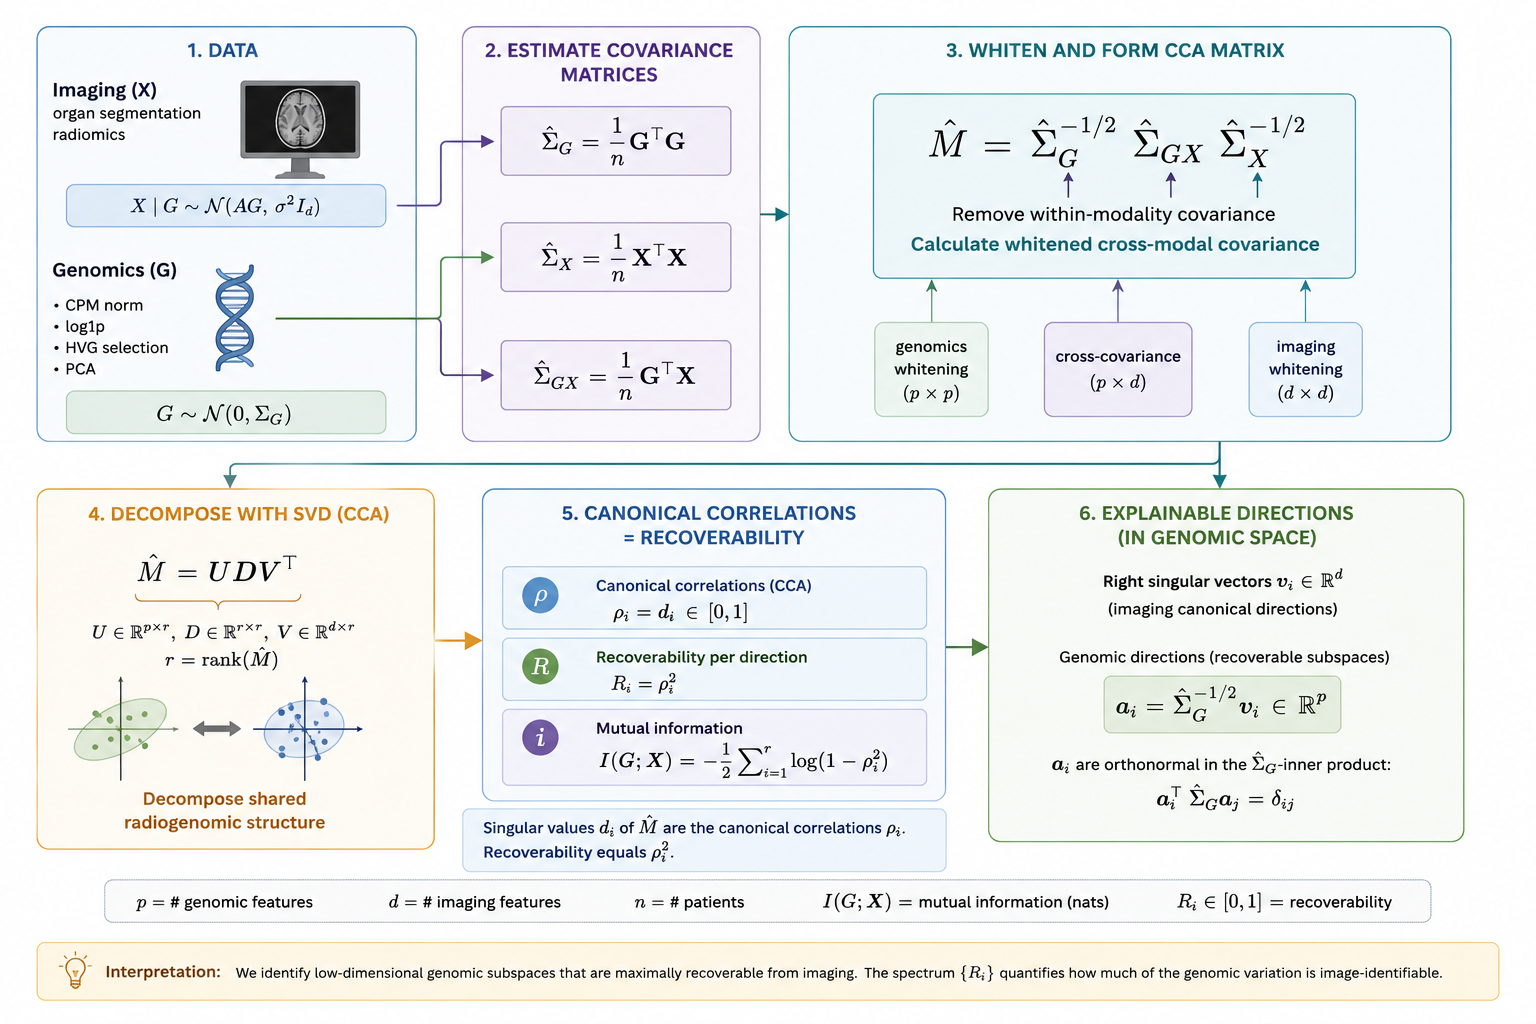
\includegraphics[width=\linewidth]{notebooks/figures/schematic/schematic.png}
\caption{Overview of the recoverability estimator. From the imaging ($X$) and
genomic ($G$) feature matrices we form regularized covariances
$\hat\Sg, \hat\Sx, \hat\Sgx$, whiten and assemble the cross-modal matrix
$\hat M = \hat\Sg^{-1/2}\hat\Sgx\hat\Sx^{-1/2}$, and take its SVD. The singular
values are the canonical correlations $\hat\rho_i$; the recoverabilities are
$\hat R_i = \hat\rho_i^2$ and the mutual information is
$I(G;X) = -\tfrac12\sum_i \log(1-\hat\rho_i^2)$; the left singular vectors map
back to image-identifiable genomic directions $\hat a_i$. The spectrum
$\{\hat R_i\}$ quantifies how much of the genomic variation is identifiable from
imaging and along how many directions.}
\label{fig:schematic}
\end{figure}

\subsection{Regularized covariances}
\label{sec:estimation-cov}
Replace sample covariances by shrinkage estimators (e.g.\ Ledoit--Wolf~\citep{ledoit2004shrinkage}),
$\hat\Sg = (1-\alpha_G)\,S_G + \alpha_G\, \nu_G I_p$ and likewise $\hat\Sx$, with
$S_G = n^{-1}\mathbf{G}\T\mathbf{G}$ the centered sample covariance; the
cross-covariance is $\hat\Sgx = n^{-1}\mathbf{G}\T\mathbf{X}$. Shrinkage keeps
$\hat\Sg, \hat\Sx$ invertible and well-conditioned, which is required for the
whitening in \eqref{eq:M}. When $p$ is very large it is practical to first
project genomics onto its top principal components (or onto curated pathway
scores), reducing $p$ to a manageable $p' \ll n$ before estimation; the rank
limit of Proposition~\ref{prop:rank} means little is lost provided $p'$ exceeds
the recoverable dimension.

\paragraph{Gaussian-copula marginals.}
The model's Gaussian prior constrains the \emph{marginals} of each feature, not
only their dependence. Radiomic descriptors in particular are badly
non-Gaussian --- heavy-tailed shape and texture statistics with excess kurtosis
in the tens (Section~\ref{sec:kirc}) --- so the raw second moments
$\hat\Sg,\hat\Sx$ are dominated by a few outlying patients and the whitening in
\eqref{eq:M} is unstable. A simple and assumption-faithful remedy is the
\emph{Gaussian-copula marginal transform}: replace each feature by its
rank mapped through the inverse normal CDF,
$\tilde M_{ij} = \Phi^{-1}\!\big(\mathrm{rank}_i(M_{\cdot j})/(n+1)\big)$, so
every marginal is exactly standard normal and only the dependence structure
(hence the canonical correlations) survives. This is the continuous-feature
analog of the latent-Gaussian construction of Section~\ref{sec:bernoulli}
and is the default applied to both modalities in the analyses below.

\subsection{Reduced-rank and ridge regression}
\label{sec:estimation-rrr}
The transfer map, if needed explicitly, is the multivariate regression of $X$ on
$G$. Ridge gives
$\hat A\T = (\mathbf{G}\T\mathbf{G} + \gamma I_p)^{-1}\mathbf{G}\T\mathbf{X}$,
and $\hat\sigma^2$ follows from the residual covariance. Imposing
$\rank(A) \le k$ (reduced-rank regression) bakes Proposition~\ref{prop:rank}
into the fit and is equivalent, up to regularization, to truncating the SVD of
$M$ at $k$ components.

\subsection{Regularized CCA}
\label{sec:estimation-cca}
The estimator used in the companion notebook solves \eqref{eq:gevp} with the
regularized covariances of Section~\ref{sec:estimation-cov}: form
$\hat M = \hat\Sg^{-1/2} \hat\Sgx \hat\Sx^{-1/2}$, take its SVD
$\hat M = \hat U \hat D \hat V\T$, and read off
$\hat\rho_i = \hat d_i$ (clipped to $[0,1)$),
$\hat R_i = \hat\rho_i^2$, genomic directions $\hat a_i = \hat\Sg^{-1/2}\hat u_i$,
imaging directions $\hat b_i = \hat\Sx^{-1/2}\hat v_i$. The Bayes-optimal
predictor and posterior covariance follow from
\eqref{eq:postmean}--\eqref{eq:postcov} with hats throughout. This is exactly
regularized CCA --- the recoverability program and CCA are the same computation.

\subsection{Probabilistic CCA: the latent-variable view}
\label{sec:estimation-pcca}
The rank limit motivates an explicit low-dimensional generative form. With a
shared latent $Z \in \R^{k}$,
\begin{equation}
Z \sim \N(0, I_k), \qquad
G = W_G Z + \mu_G + \epsilon_G, \qquad
X = W_X Z + \mu_X + \epsilon_X,
\label{eq:pcca}
\end{equation}
$\epsilon_G \sim \N(0, \Psi_G)$, $\epsilon_X \sim \N(0, \Psi_X)$ independent
(probabilistic CCA;~\citealp{bach2005pcca}). Here $k$ \emph{is} the dimension of
the image-identifiable genomic subspace, $Z$ is the shared biological state, and
$\epsilon_G, \epsilon_X$ are modality-private variation. The implied moments are
$\Sg = W_G W_G\T + \Psi_G$, $\Sx = W_X W_X\T + \Psi_X$,
$\Sgx = W_G W_X\T$; the maximum-likelihood loadings are the canonical directions
scaled by the canonical correlations, recovering Section~\ref{sec:estimation-cca}.
The model is fit by EM, which also yields posterior latent estimates
$\E[Z \mid x]$ and naturally accommodates anisotropic (per-feature) noise, unlike
the isotropic $\sigma^2 I_d$ of the base model.

\subsection{Sample-size regimes and dimensional collapse}
\label{sec:estimation-regimes}
Equations~\eqref{eq:postmean}--\eqref{eq:gevp} are population identities; the
estimators of Sections~\ref{sec:estimation-cov}--\ref{sec:estimation-pcca}
inherit a finite-sample bias whose magnitude is governed entirely by the
aspect ratios $p/n$ and $d/n$. The bias is not benign, and below a critical
sample size the recoverability spectrum breaks down in a specific, predictable
way.

\paragraph{Three regimes.} Let $p^\star, d^\star$ be the working dimensions
after any pre-reduction (e.g.\ PCA), and write $\kappa_G = p^\star/n$,
$\kappa_X = d^\star/n$.
\begin{enumerate}
\item \emph{Classical} ($\kappa_G + \kappa_X \ll 1$). Sample CCA is consistent;
$\hat\rho_i \to \rho_i$ at the usual $n^{-1/2}$ rate and the in-sample spectrum
is a faithful estimate of the population one.
\item \emph{High-dimensional} ($\kappa_G + \kappa_X \lesssim 1$, both bounded
away from $1$). Under the null $\Sgx = 0$, the squared sample canonical
correlations follow a Wachter-type law on
$[(\sqrt{\kappa_G(1-\kappa_X)} - \sqrt{\kappa_X(1-\kappa_G)})^2,
 (\sqrt{\kappa_G(1-\kappa_X)} + \sqrt{\kappa_X(1-\kappa_G)})^2]$
\citep{wachter1980limiting,yang2015independence}; the leading sample value already sits well
above zero by geometry. Estimates of $\rho_i$ are systematically inflated and
ordinary CCA must be replaced by its regularized form, with shrinkage
parameters tuned by cross-validation.
\item \emph{Saturating} ($p^\star + d^\star \ge n$). The rows of $\mathbf{G}$
and $\mathbf{X}$ live in subspaces whose intersection has dimension at least
$p^\star + d^\star - n + 1$; consequently
$\hat\rho_1 = \cdots = \hat\rho_q = 1$ for $q = \min(p^\star, d^\star) - (n -
\max(p^\star, d^\star))_+$ \emph{regardless of any underlying association}.
The empirical mutual information diverges, the in-sample
$\tr(\hat\Sgx \hat\Sx^{-1} \hat\Sxg)/\tr(\hat\Sx)$ approaches the rank fraction
of the genomic span, and the permutation null collapses onto the observed
value (its $p$-values concentrate near $1$). Nothing in the spectrum is
estimable in this regime without shrinkage \emph{plus} dimension reduction;
shrinkage alone keeps the matrices invertible but does not restore
identifiability.
\end{enumerate}

\paragraph{Quantitative warning signs.} Three diagnostics, jointly, separate
real signal from dimensional artifact:
\begin{itemize}
\item the gap between in-sample $\hat R_i$ and the $K$-fold value $\hat
R_i^{\mathrm{cv}}$; under regime~3 this gap approaches $\hat R_i - 0$;
\item the permutation null for $\hat\rho_1$: if the observed value lies inside
the bulk, the result is consistent with chance;
\item the cross-validated $R^2$ of the leading canonical score $a_1\T g$
predicted from $x$ on a held-out split; in regime~3 it is typically large and
\emph{negative} (worse than predicting the mean), a behavior seen empirically
on TCGA-KIRC at $n=131$ with $p^\star = 100, d^\star = 107$ in the companion
notebook.
\end{itemize}

\paragraph{Recommendations.} Choose $p^\star$ and $d^\star$ \emph{adaptively
from $n$}, not from the native modality dimensions:
\begin{itemize}
\item Target $p^\star + d^\star \le n/\tau$ with $\tau \ge 5$ as a working
rule (we use $p^\star, d^\star \le \lfloor n/\tau \rfloor$ per side in the
notebook; $\tau \in [5,10]$ trades bias for resolution). Reduce both
modalities by PCA when needed --- reducing only the larger side leaves the
estimator in regime~3.
\item Treat $\hat R_i^{\mathrm{cv}}$ (Section~\ref{sec:estimation-honest}) as
the primary estimand and report the in-sample $\hat R_i$ only with the gap
made explicit; the in-sample fraction of imaging variance attributable to
genomics should be reported alongside a cross-validated counterpart, e.g.\
$\sum_i \hat R_i^{\mathrm{cv}}/\min(p^\star, d^\star)$.
\item Power planning. The leading population correlation $\rho_1$ is detectable
above the Wachter bulk only when its squared value exceeds
$(\sqrt{\kappa_G(1-\kappa_X)} + \sqrt{\kappa_X(1-\kappa_G)})^2$; solving for $n$
gives a minimum sample size given a hypothesized effect. For
$\rho_1^2 = 0.2$ and a balanced $p^\star = d^\star$, this requires roughly
$n \gtrsim 25\,p^\star$, an order of magnitude beyond what cohort sizes in
radiogenomics usually offer --- reinforcing the need for aggressive
pre-reduction.
\item Probabilistic CCA (Section~\ref{sec:estimation-pcca}) with a small,
fixed latent dimension $k$ is the most parsimonious option when $n$ is the
binding constraint; rank-$k$ regularization sidesteps the high-dimensional
bulk by construction.
\end{itemize}

The practical message is conservative: in radiogenomic cohorts, sample size
is almost always the binding constraint and a defensible analysis is the one
whose effective $p^\star + d^\star$ is a small fraction of $n$, with both
sides reduced symmetrically and every reported number a cross-validated or
permutation-calibrated one.

Figure~\ref{fig:synthetic-sweep} illustrates these regimes on the synthetic
instance, where the planted truth is known. As $n$ grows with $p^\star, d^\star$
scaled to keep $\kappa_G + \kappa_X$ bounded, the in-sample $\hat\rho_1$ sits at
or near $1$ across the small-$n$ saturating regime --- indistinguishable from
the permutation null --- while the cross-validated $\hat R_1^{\mathrm{cv}}$ only
separates from zero once $n$ clears the Wachter edge. The empirical mutual
information shows the same threshold behavior.

\begin{figure}[h]
\centering
\includegraphics[width=0.85\linewidth]{\synfig{sample_complexity_sweep.pdf}}
\caption{Sample-complexity sweep on the synthetic instance with known truth.
In-sample $\hat\rho_1$ tracks the null until $n$ exceeds the Wachter edge;
cross-validated $\hat R_1^{\mathrm{cv}}$ and empirical $\hat I(G;X)$ only
become informative past that threshold. Compare to
Figure~\ref{fig:kirc-sweep} for the same diagnostic on TCGA-KIRC.}
\label{fig:synthetic-sweep}
\end{figure}

The sweep above grows $p^\star, d^\star$ with $n$, which entangles ``more data''
with ``bigger model''. The complementary question --- how much data is needed at
a \emph{fixed} model --- is answered by Figure~\ref{fig:synthetic-downsample},
which holds $p^\star = d^\star = 20$ and varies only $n$ on the same synthetic
instance, whose planted leading recoverability $\rho_1^2 = 0.65$ is known in
closed form (Proposition~\ref{prop:eig}). Two thresholds separate. The
cross-validated \emph{point} estimate $\hat R_1^{\mathrm{cv}}$ is already close to
the truth at small $n$ (within $90\%$ by $n\approx 80$, i.e.\ $n\approx 2(p^\star
+ d^\star)$), because the planted signal is strong. But the estimate cannot be
\emph{certified} against the permutation null until later: the null $95\%$
quantile is inflated to $\approx 1$ in the saturating regime
($n \lesssim p^\star + d^\star$) and only decays below the estimate at
$n\approx 176 \approx 4.4(p^\star + d^\star)$. The practical reading is that
``how much data'' depends on the claim: recovering the right number takes far
less data than proving it is not an artifact of the high-dimensional geometry,
and the cohort downsample sweeps (Sections~\ref{sec:adni-datasize}) report the
latter, conservative threshold.

\begin{figure}[h]
\centering
\includegraphics[width=0.85\linewidth]{\synfig{synthetic_downsample_recoverability.pdf}}
\caption{Fixed-model downsampling sweep on the synthetic instance ($p^\star =
d^\star = 20$, planted $\rho_1^2 = 0.65$). The cross-validated estimate (blue)
tracks the known truth (green) even at small $n$, but the permutation null
$95\%$ quantile (red, dashed) is saturated near $1$ in the small-$n$ regime and
only falls below the estimate at $n\approx 176$. Recovering the value needs less
data than certifying it. Companion to the growing-model sweep of
Fig.~\ref{fig:synthetic-sweep} and the cohort sweeps
(Fig.~\ref{fig:adni-datasize}).}
\label{fig:synthetic-downsample}
\end{figure}

\subsection{Honest recoverability: cross-validation and permutation}
\label{sec:estimation-honest}
In-sample canonical correlations are biased upward, severely so when $p, d$ are
not small relative to $n$. Two safeguards, both implemented in the notebook:
\begin{itemize}
\item \emph{Cross-validation.} Estimate $\hat a_i, \hat b_i$ on a training fold;
on the held-out fold form the scores $\hat a_i\T g$ and $\hat b_i\T x$ and report
their out-of-sample squared correlation as the honest $\hat R_i$. The gap to the
in-sample value quantifies overfitting.
\item \emph{Permutation test.} Repeatedly permute the patient labels of one
modality, refit, and collect the leading canonical correlation to build a null
distribution; the permutation $p$-value tests whether any genomic direction is
image-identifiable beyond chance.
\end{itemize}

\paragraph{Scale-matched effective rank.}
A subtlety arises when these two safeguards are combined to count
\emph{how many} directions are identifiable. The in-sample permutation null
of the leading $\hat\rho_1$ is itself inflated toward $1$ by the
high-dimensional geometry of Section~\ref{sec:estimation-regimes}, whereas
$\hat R_i^{\mathrm{cv}}$ is honestly deflated; thresholding the deflated
statistic against the inflated null forces the estimated rank to zero
regardless of any true signal. The two must be compared on the same scale. We
therefore build the null of the \emph{cross-validated} statistic directly:
permute patient labels, recompute the full $K$-fold $\hat R_i^{\mathrm{cv}}$,
and define the \emph{effective image-identifiable rank} as the number of
directions whose observed $\hat R_i^{\mathrm{cv}}$ exceeds its own
permutation $95\%$ quantile at permutation $p<0.05$. This is the estimand we
report below.

Figure~\ref{fig:synthetic-cv} shows both diagnostics on the synthetic instance.
The in-sample $\hat R_i$ overshoots the planted truth by the amount predicted
by the high-dimensional bias, while the $5$-fold $\hat R_i^{\mathrm{cv}}$
tracks the truth for identifiable directions and collapses toward the null
$95\%$ quantile thereafter. Figure~\ref{fig:synthetic-perm} shows the
permutation null on $\hat\rho_1$: when the true signal is nonzero, the
observed value sits cleanly outside the null bulk and the per-direction
$p$-values fall below $0.01$ for the top three components, matching the
planted rank.

\begin{figure}[h]
\centering
\includegraphics[width=0.85\linewidth]{\synfig{cv_recoverability.pdf}}
\caption{Cross-validated recoverability on a synthetic instance with planted
rank $k=6$ (the sixth correlation near zero). In-sample $\hat R_i$ (gray) is
biased upward; $5$-fold
$\hat R_i^{\mathrm{cv}}$ (blue) tracks the planted truth for the identifiable
directions and collapses to the null floor afterwards.}
\label{fig:synthetic-cv}
\end{figure}

\begin{figure}[h]
\centering
\includegraphics[width=0.75\linewidth]{\synfig{permutation_null.pdf}}
\caption{Permutation null on the leading canonical correlation
$\hat\rho_1$ for the synthetic instance. Red marks the observed value;
$p < 0.01$ for the top three directions, recovering the planted rank.}
\label{fig:synthetic-perm}
\end{figure}

The same optimism appears in the aggregate fraction of imaging variance
attributable to genomics. Figure~\ref{fig:synthetic-vardecomp} shows the
in-sample share $\sum_i \hat R_i / \min(p^\star, d^\star)$ alongside its
cross-validated counterpart on the synthetic instance: the in-sample number
sits well above the planted truth while the CV value tracks it. The same
diagnostic on TCGA-KIRC (Section~\ref{sec:kirc}) reports
$0.193$ in-sample against $0.012$ cross-validated --- a sixteen-fold gap that
is consistent with the synthetic mechanism rather than with any genuinely
recoverable signal.

\begin{figure}[h]
\centering
\includegraphics[width=0.75\linewidth]{\synfig{imaging_variance_decomposition.pdf}}
\caption{Share of imaging variance attributable to genomics on the synthetic
instance: in-sample (gray) versus $5$-fold cross-validated (blue), with the
planted truth marked. The in-sample share is biased upward by the
high-dimensional inflation described in
Section~\ref{sec:estimation-regimes}.}
\label{fig:synthetic-vardecomp}
\end{figure}

\subsection{Checking the model assumptions}
\label{sec:assumption-checks}
The closed-form recoverability and mutual information are exact \emph{under} the
linear--Gaussian law; before trusting the numbers we verify, upfront, how far
each cohort departs from it. Three checks bracket the assumptions the estimator
actually uses.

\paragraph{(i) Marginal and joint Gaussianity.}
The Gaussian-copula transform (Section~\ref{sec:estimation-cov}) makes every
\emph{marginal} exactly normal by construction; the question is whether the
\emph{joint} $[G_{\mathrm{pca}}, X_{\mathrm{pca}}]$ is. We test it with a
Mahalanobis-distance QQ plot against the $\chi^2_p$ law (squared Mahalanobis
distances are $\chi^2_p$ under joint MVN) and Mardia's standardized skew/kurtosis
ratios (Fig.~\ref{fig:mvn-joint}). Per-modality marginal normality does not
imply joint normality, so this is the assumption the spectrum genuinely relies
on.

\paragraph{(ii) Linearity of the dependence.}
Canonical correlation sees only second-order (linear) coupling. We complement it
with the distance correlation~\citep{szekely2007dcor}, which is zero \emph{iff}
$G_{\mathrm{pca}}$ and $X_{\mathrm{pca}}$ are independent and therefore detects
non-linear and higher-order dependence the linear--Gaussian estimator is blind
to. We report a permutation $p$-value (the statistic has a positive
finite-sample bias, so its null, not its raw value, is the reference). A
significant distance correlation where the cross-validated recoverability is
null would indicate a channel the linear bound understates.

\paragraph{(iii) Per-feature marginals.}
As documentation of the copula step, we summarize per-feature skewness and excess
kurtosis on the raw features and confirm both vanish after the transform.

\begin{figure}[h]
\centering
\includegraphics[width=0.55\linewidth]{\synfig{mvn_joint_diagnostic.pdf}}
\caption{Joint-MVN check on the concatenated working-space scores
$[G_{\mathrm{pca}}, X_{\mathrm{pca}}]$ for the synthetic instance: squared
Mahalanobis distances against $\chi^2_p$ quantiles lie on the line, with kurtosis
ratio $\approx 1$ and a $0.4\%$ tail beyond the $99\%$ shell. The real cohorts
(Fig.~\ref{fig:mvn-joint-real}) depart from this in their upper tails.}
\label{fig:mvn-joint}
\end{figure}

\begin{figure}[h]
\centering
\begin{minipage}{0.32\linewidth}\centering
\includegraphics[width=\linewidth]{\kircfig{mvn_joint_diagnostic.pdf}}\\
{\footnotesize (a) TCGA-KIRC}
\end{minipage}\hfill
\begin{minipage}{0.32\linewidth}\centering
\includegraphics[width=\linewidth]{\nsclcfig{mvn_joint_diagnostic.pdf}}\\
{\footnotesize (b) NSCLC}
\end{minipage}\hfill
\begin{minipage}{0.32\linewidth}\centering
\includegraphics[width=\linewidth]{\adnifig{mvn_joint_diagnostic.pdf}}\\
{\footnotesize (c) ADNI}
\end{minipage}
\caption{Joint-MVN QQ plots on the three real cohorts (squared Mahalanobis
distances of $[G_{\mathrm{pca}}, X_{\mathrm{pca}}]$ vs.\ $\chi^2_p$ quantiles;
the line $y=x$ is exact joint Gaussianity). The copula makes every marginal
Gaussian, so departures here are purely \emph{joint} non-Gaussianity. All three
track the line through the bulk and lift above it in the upper tail --- the
residual leptokurtosis (heavy joint tails) quantified in
Table~\ref{tab:assumptions}. The deviation is largest in the small tumor
cohorts (a,~b) and mildest in ADNI (c), the cohort with the most favorable
$n/(\dim G + \dim X)$ ratio, consistent with the part of the inflation that is
finite-sample. Together with the synthetic ideal (Fig.~\ref{fig:mvn-joint}) these
panels are the visual companion to the assumption table.}
\label{fig:mvn-joint-real}
\end{figure}

\paragraph{Findings.}
Table~\ref{tab:assumptions} collects the three checks across cohorts. Two
patterns are robust. First, the copula transform is doing real work: raw genomic
marginals are severely non-Gaussian ($78\%$ of KIRC probes fail $|\mathrm{skew}|
\le 2,\ |\mathrm{kurt}| \le 7$, median excess kurtosis $70$), and all go to
$0\%$ afterwards. Second, and less obviously, \emph{marginal Gaussianity does not
buy joint Gaussianity}: even post-copula, the share of samples beyond the
$\chi^2$ $99\%$ shell is $7$--$16\%$ rather than the nominal $1\%$. Part is
finite-sample (the ratio $n/(\dim G + \dim X) \approx 2.5$ in all three inflates
the Mahalanobis tail), but it shrinks monotonically with $n$
($16\% \to 12\% \to 8\%$ for KIRC $\to$ NSCLC $\to$ ADNI), implicating genuine
residual \emph{tail dependence} the copula cannot remove. The Mardia skew ratio
stays $\approx 0$, so the joint is symmetric but leptokurtic. The distance
correlation is significant in every cohort ($p = 0.005$) but only modestly above
its inflated null, and its ordering tracks the \emph{linear} recoverability
rather than exceeding it --- there is no cohort where non-linear dependence
lights up while the linear channel is dead.

\begin{table}[h]
\centering
\small
\begin{tabular}{lccc}
\toprule
 & TCGA-KIRC & NSCLC & ADNI \\
\midrule
$n$ / joint dim                       & $190/76$ & $129/50$ & $702/280$ \\
Joint kurt.\ ratio ($1$ = MVN)         & $1.17$   & $1.14$   & $1.02$ \\
Tail beyond $\chi^2_{.99}$ ($1\%$ = MVN) & $15.8\%$ & $12.4\%$ & $8.1\%$ \\
Genomic marginals non-normal (raw $\to$ post) & $78\%\!\to\!0\%$ & $57\%\!\to\!0\%$ & $24\%\!\to\!0\%$ \\
Distance corr.\ (obs / null$_{95}$ / $p$) & $0.43/0.37/.005$ & $0.34/0.31/.005$ & $0.32/0.27/.005$ \\
\bottomrule
\end{tabular}
\caption{Model-assumption diagnostics. The copula removes all marginal
non-normality; the joint remains mildly heavy-tailed (worst in the small tumor
cohorts, near-Gaussian in ADNI); the distance correlation reveals no non-linear
channel beyond the linear one.}
\label{tab:assumptions}
\end{table}

\paragraph{What this does and does not cost the upper bound.}
It is worth separating two claims that the phrase ``$I(G;X)$ is an upper bound''
can mean. The \emph{operational} bound --- that no estimator, linear or
non-linear, can recover $G$ from $X$ better than $I(G;X)$ allows --- is the data
processing inequality $G \to X \to \hat g(X)$ and holds for the \emph{true} joint
law regardless of its shape (Section~\ref{sec:bern-mi}). What requires Gaussianity
is the second, computational claim: that the \emph{number} we report,
$-\tfrac12\sum_i\log(1-\hat\rho_i^2)$, equals that true $I(G;X)$. The copula
secures the marginals; the residual joint non-Gaussianity above means the two are
equal only approximately. Crucially, the mis-specification is one-sided in a
favorable direction: because canonical correlation captures only linear
coupling, ignoring higher-order dependence can only make the Gaussian formula
\emph{under}-count the true $I(G;X)$, never over-count it --- so the reported
figure is conservative as a statement about the true channel, not optimistic.
The distance-correlation check bounds how much is being missed (little), and the
finite-sample optimism that runs the \emph{other} way is removed separately by
the permutation-calibrated upper confidence limit
(Section~\ref{sec:kirc-ucb}). The net reading: significance and the
identifiable-rank conclusions are distribution-free and stand; the MI
\emph{magnitudes} are best read as approximate, most trustworthy in ADNI
(near-Gaussian joint, large $n$) and most caveated in the small, heavier-tailed
tumor cohorts.

\paragraph{A signed bias, made precise.}
The favorable direction is not heuristic; the copula pins it down. Write
$I(G;X) = h(G) + h(X) - h(G,X)$. The copula forces each marginal to be exactly
Gaussian, so $h(G)$ and $h(X)$ equal their Gaussian values and the \emph{only}
term in which the true law can differ from the Gaussian surrogate is the joint
entropy $h(G,X)$. Because the Gaussian is the maximum-entropy law for a fixed
covariance, $h(G,X) \le h_{\mathrm{gauss}}(G,X)$, whence
\begin{equation}
I(G;X) - \Bigl(-\tfrac12{\textstyle\sum_i}\log(1-\rho_i^2)\Bigr)
\;=\; h_{\mathrm{gauss}}(G,X) - h(G,X) \;\ge\; 0,
\label{eq:mi-lower-bound}
\end{equation}
with equality \emph{iff} the joint is Gaussian. So, given Gaussian marginals,
the population canonical-correlation mutual information is a genuine \emph{lower}
bound on the truth --- exact under joint Gaussianity, an under-estimate
otherwise --- and the gap is precisely the non-Gaussian (non-linear,
higher-order) dependence that CCA cannot see, which is what the distance
correlation probes. (Without the Gaussian-marginal condition the marginal
negentropies re-enter \eqref{eq:mi-lower-bound} and the sign is no longer
guaranteed; securing this clean direction is a concrete reason to apply the
copula.) The two error sources therefore push in \emph{opposite} directions:
population mis-specification can only \emph{lower} the estimate relative to the
true $I(G;X)$, while finite-sample inflation of $\hat\rho_i$ \emph{raises} it.
The permutation-calibrated upper confidence limit
(Section~\ref{sec:kirc-ucb}) controls the second; \eqref{eq:mi-lower-bound} and
the distance-correlation check bound the first. A reported figure that is small
after both controls is therefore a trustworthy statement that the channel is
genuinely narrow, not an artifact of either bias.

\section{Interpretation for radiogenomics}
\label{sec:interpretation}

The model reframes the radiogenomic
question~\citep{rutman2009radiogenomics,gillies2016radiomics,lambin2017radiomics,bodalal2019radiogenomics}.
Rather than testing whether CT
predicts each gene --- a high-dimensional, low-power multiple-testing problem ---
it asks for the \emph{recoverability spectrum} $\{\rho_i^2\}$ and the associated
genomic directions $\{a_i\}$. The outputs are: (1) a small number of
image-identifiable genomic axes, with gene/pathway loadings that make them
biologically legible; (2) a hard bound $\Sgcx$ on what any predictor can achieve,
per direction; (3) a total information budget $I(G;X)$; and (4) an honest,
cross-validated estimate of each. The governing principle is that radiogenomics
should target \emph{image-identifiable low-dimensional genomic subspaces}, whose
dimension is set by the biology--imaging channel and not by the gene panel size.

Section~\ref{sec:attainable} adds the fifth and, for a practitioner, the most
consequential output: (5) a ceiling $\mathcal{I}_n$ on how much of that budget a
cohort of size $n$ can actually claim. The four quantities above are properties
of the biology--imaging channel; $\mathcal{I}_n$ is a property of the
\emph{study}. Reporting it changes what a null result means. A per-gene AUC of
$0.66$ is uninformative in isolation, but against an attainable ceiling of
$0.76$ it is most of what the cohort had to give, whereas against a
ceiling of $0.95$ it is a failure of the predictor. Three practical rules follow
directly:
\begin{itemize}
\item \emph{Report bits, not just $p$-values.} $\mathcal{I}_n$ is on a scale a
clinician can price --- one bit is one perfectly measured balanced binary
biomarker --- and it is comparable across disease, modality and cohort.
\item \emph{Size the study from Eq.~\eqref{eq:design-n}, not from convention.}
The learning cost $\nu = d^\star/\mathrm{SNR}$ makes the imaging representation
a design variable on the same footing as the patient count, and
Corollary~\ref{cor:optimal-d} says the best feature budget is finite.
\item \emph{Prefer a short, pre-specified gene panel.} By
Corollary~\ref{cor:quartic} the directions a wider panel adds are exactly the
weak ones a finite cohort cannot certify, and empirically
(Section~\ref{sec:anchor-results}) a four-gene panel carries most of what the
one cohort with a robust channel can deliver.
\end{itemize}

\section{A Bernoulli extension for mutation data via a Gaussian copula}
\label{sec:bernoulli}

The linear--Gaussian model of Section~\ref{sec:setup} is well matched to
continuous, approximately log-normal genomic readouts: log-CPM gene expression,
methylation $\beta$- or $M$-values, log-CNV ratios. It is plainly misspecified
for somatic mutation calls, where each $G_j \in \{0,1\}$ indicates the presence
of a non-silent variant in gene $j$ and the marginal frequencies $p_j$ are
small, gene-specific, and highly heterogeneous. This section extends the
framework to such data by replacing the Gaussian prior on $G$ with a
\emph{Gaussian-copula Bernoulli} (equivalently, multivariate probit) prior,
while preserving the canonical-correlation / mutual-information machinery of
Sections~\ref{sec:mi}--\ref{sec:canonical}.

\subsection{The latent-Gaussian generative model}
\label{sec:bern-model}

Let $p_j = \Pr(G_j = 1)$ and $\tau_j = \Phi^{-1}(1-p_j)$, where $\Phi$ is the
standard normal CDF. Introduce a latent vector
\[
  Z \sim \mathcal N(0, \Sigma_Z), \qquad
  \mathrm{diag}(\Sigma_Z) = I_p,
\]
and define the observed mutation indicator by thresholding:
\[
  G_j = \mathbf{1}\!\{Z_j > \tau_j\}, \qquad j = 1,\ldots,p.
\]
By construction the marginals are correct, $G_j \sim \mathrm{Bern}(p_j)$, and
the pairwise joint laws are governed by the tetrachoric correlation $\Sigma_{Z,jk}$,
which can be any positive-definite correlation matrix --- providing arbitrary
dependence structure between mutated genes (e.g.\ mutual exclusivity,
co-occurrence within pathways).

Imaging is coupled to the \emph{latent} state, not to the indicators directly:
\begin{equation}
  X \mid Z \sim \mathcal N\!\bigl(B\,Z,\ \sigma^2 I_d\bigr),
  \qquad
  B \in \R^{d \times p}.
  \label{eq:bern-channel}
\end{equation}
This is the natural specification: the biological mechanism that produces an
imageable phenotype (proliferation, vascularity, necrosis) responds to an
underlying continuous burden, of which an observed mutation is a coarse,
binarized readout. The joint structure factors as
\[
  Z \to G,\qquad Z \to X,
\]
so $G$ and $X$ are conditionally independent given $Z$.

\subsection{Mutual information and a tight DPI bound}
\label{sec:bern-mi}

Because $G$ is a deterministic, memoryless function of $Z$, the data
processing inequality yields the upper bound
\begin{equation}
  I(G;X) \;\le\; I(Z;X),
  \label{eq:bern-dpi}
\end{equation}
with equality only if $Z$ can be recovered from $G$ (impossible whenever any
$p_j \in (0,1)$, since thresholding is lossy). The right-hand side reduces
exactly to the Gaussian formula of Section~\ref{sec:mi}: if $\{\rho_i\}_{i=1}^{k}$
denote the canonical correlations of $(Z,X)$ under \eqref{eq:bern-channel}, then
\begin{equation}
  I(Z;X) \;=\; -\tfrac{1}{2}\sum_{i=1}^{k} \log\bigl(1-\rho_i^2\bigr),
  \qquad
  k = \rank\bigl(\Sigma_Z^{1/2} B^\top \Sigma_X^{-1} B \Sigma_Z^{1/2}\bigr),
  \label{eq:bern-mi}
\end{equation}
with $\Sigma_X = B \Sigma_Z B^\top + \sigma^2 I_d$. The recoverability spectrum,
the directions $\{a_i\}$, and the eigenproblem of
Section~\ref{sec:eigenproblem} all transfer verbatim, with $\Sigma_G$ replaced
by $\Sigma_Z$.

\paragraph{The binarization gap.}
The slack in \eqref{eq:bern-dpi} is
\[
  I(Z;X) - I(G;X) \;=\; H(Z\mid G) - H(Z\mid G,X) \;=\; I(Z;X \mid G),
\]
the residual information about $Z$ not already revealed by the mutation call.
For a single gene with frequency $p_j$, the entropy lost to binarization is
$H(Z_j) - H(G_j) = \tfrac12 \log(2\pi e) - h_2(p_j)$ where $h_2$ is the binary
entropy in nats; rare mutations ($p_j \ll 1/2$) are highly lossy, common ones
near $p_j = 1/2$ less so. Thus \eqref{eq:bern-dpi} is tightest for cohorts
dominated by intermediate-frequency mutations and loosest for rare-variant
panels --- a useful guide to when the bound is informative.

\subsection{Per-gene recoverability and AUC ceilings}
\label{sec:bern-pergene}

For a named mutation $G_j$, the Bayes-optimal predictor from $X$ is the
posterior probability
\[
  \pi_j(x) \;=\; \Pr(G_j = 1 \mid X = x) \;=\; \Phi\!\left(\frac{\mu_j(x) - \tau_j}{s_j}\right),
\]
where $(\mu_j(x), s_j^2) = (\E[Z_j \mid X=x],\ \Var(Z_j \mid X=x))$ are the
linear-Gaussian posterior moments for the latent coordinate, computed from
$(\Sigma_Z, B, \sigma^2)$ exactly as in Section~\ref{sec:posterior}. The
\emph{latent recoverability} $R_j^Z = \Var(\E[Z_j\mid X]) / \Var(Z_j)$ is the
direct analog of $R(v)$ in the Gaussian case, and the binary AUC of any
predictor $\hat G_j(x)$ is bounded by
\begin{equation}
  \mathrm{AUC}_j \;\le\; \tfrac12+\tfrac{2}{\pi}\arcsin\!\sqrt{R_j^Z/2},
  \label{eq:bern-auc}
\end{equation}
attained by the Bayes score $\pi_j(x)$ when $G_j$ is binarized at its median
($p_j=\tfrac12$). The right-hand side is the trivariate Gaussian orthant
probability $\Pr(\mu_j(x_1)>\mu_j(x_0)\mid Z_{j,1}>0,\,Z_{j,0}\le0)$ and is the
least favorable prevalence: a feature binarized away from its median admits a
higher Bayes AUC at the same $R_j^Z$, so \eqref{eq:bern-auc} is a valid ceiling
only for median splits and is conservative elsewhere. Equation~\eqref{eq:bern-auc}
is the natural object to compare against the empirical per-gene
$\mathrm{AUC}_{\mathrm{LR}}$ and $\mathrm{AUC}_{\mathrm{RF}}$ of
Section~\ref{sec:kirc-pergene}: an empirical AUC near $0.5$ is consistent with
either a small $R_j^Z$ \emph{or} a degenerate $p_j$, and \eqref{eq:bern-auc}
disentangles the two.

\subsection{Estimation}
\label{sec:bern-estimation}

The estimator splits into three independent pieces, each well-studied:

\begin{enumerate}
\item[(i)] \textbf{Marginal thresholds.} Estimate $\hat p_j = \bar G_{\cdot j}$
and set $\hat\tau_j = \Phi^{-1}(1-\hat p_j)$. Apply a continuity correction or
empirical-Bayes shrinkage for rare mutations.
\item[(ii)] \textbf{Latent correlation $\hat\Sigma_Z$.} Estimate pairwise
tetrachoric correlations from $2{\times}2$ tables of $(G_j, G_k)$ by maximum
likelihood under the bivariate-normal copula, then project the resulting matrix
to the nearest positive-definite correlation matrix (e.g.\ Higham's
\texttt{nearcorr}~\citep{higham2002nearcorr}). For high-dimensional panels apply Ledoit--Wolf shrinkage as
in Section~\ref{sec:estimation-cov}.
\item[(iii)] \textbf{Cross-modal covariance $\hat\Sigma_{ZX}$.} The
point-biserial covariance $\Cov(G_j, X_\ell)$ is related to the latent
covariance by
\[
  \Cov(G_j, X_\ell) \;=\; \phi(\tau_j)\,\Cov(Z_j, X_\ell),
\]
where $\phi$ is the standard normal density. Estimate $\Cov(G_j,X_\ell)$ from
the sample and rescale by $\phi(\hat\tau_j)$ to obtain $\hat\Sigma_{ZX, j\ell}$.
\end{enumerate}

With $(\hat\Sigma_Z, \hat\Sigma_{ZX}, \hat\Sigma_X)$ in hand, the regularized
CCA of Section~\ref{sec:estimation-cca}, the permutation null of
Section~\ref{sec:estimation-honest}, and the empirical MI bound
(estimated, e.g., by $k$-nearest-neighbor or neural
estimators~\citep{kraskov2004mi,belghazi2018mine,paninski2003entropy}) carry over
without further change. The dimensional-collapse warnings of
Section~\ref{sec:estimation-regimes} are if anything \emph{more} acute, since
tetrachoric estimation has higher variance than Pearson correlation,
particularly for rare-rare gene pairs.

\subsection{Mixed-modality genomics}
\label{sec:bern-mixed}

In practice a single cohort carries both continuous (expression, CNV) and
binary (mutation) features. The copula formulation accommodates this by
partitioning the latent vector as $Z = (Z^{\mathrm{cts}}, Z^{\mathrm{bin}})$
with a single joint $\Sigma_Z$. The continuous block uses the identity link
($G^{\mathrm{cts}} = Z^{\mathrm{cts}}$ up to marginal standardization) and the
binary block uses the probit link of Section~\ref{sec:bern-model}. Estimation
of $\Sigma_Z$ proceeds blockwise --- Pearson within the continuous block,
tetrachoric within the binary block, polyserial across blocks --- after which
the rest of the pipeline is identical. This is the route by which the present
manuscript's gene-expression analysis (Section~\ref{sec:tcga-kirc}) and the
per-gene mutation validation (Section~\ref{sec:kirc-pergene}) can be unified
into a single coherent recoverability calculation.

\section{Anchor genes: how much of the channel is a handful of genes?}
\label{sec:anchors}

The ceiling says imaging can support only a few genomic directions at realistic
$n$. It does not say \emph{which}. A radiologist's operational question is
sharper: if the recoverable subspace is small, is it spanned by genes we already
know about?

Let $\mathcal{A}\subset\{1,\dots,p\}$ be a hand-specified anchor panel --- the
canonical drivers and lineage markers of the disease. The chain rule splits the
channel information exactly,
\begin{equation}
I(G;X) \;=\; I(G_\mathcal{A};X) \;+\; I(G_{\bar{\mathcal{A}}};X \mid G_\mathcal{A}),
\label{eq:chainrule}
\end{equation}
and under the joint Gaussian law the conditional term is an ordinary mutual
information between residualized variables: with
$G^{\perp}_{\bar{\mathcal{A}}} = G_{\bar{\mathcal{A}}}
 - \Sigma_{\bar{\mathcal{A}}\mathcal{A}}\Sigma_{\mathcal{A}}^{-1}G_\mathcal{A}$
and $X^{\perp} = X - \Sigma_{X\mathcal{A}}\Sigma_{\mathcal{A}}^{-1}G_\mathcal{A}$,
\begin{equation}
I(G_{\bar{\mathcal{A}}};X\mid G_\mathcal{A})
= I\big(G^{\perp}_{\bar{\mathcal{A}}};\,X^{\perp}\big),
\label{eq:conditional-mi}
\end{equation}
computable by the same CCA machinery. Operationally this is Gram--Schmidt in the
$\Sg$ metric: the genomics matrix is whitened \emph{against the anchors}, so
that ``new information'' means new relative to the panel rather than merely
correlated with it. Without this step the pervasive co-expression structure of
the transcriptome would credit the residual block with information the anchors
already carry.

\begin{definition}[Anchor sufficiency]
\label{def:anchor-suff}
$\eta(\mathcal{A}) := I(G_\mathcal{A};X)\,/\,I(G;X)\in[0,1]$, with the
finite-sample counterpart $\eta_n(\mathcal{A})$ obtained by replacing both
terms with their attainable versions \eqref{eq:attainable-info}.
\end{definition}

Two features of $\eta_n$ deserve emphasis. First, it is the right currency for
the question: a panel that captures $80\%$ of the \emph{channel} but requires
$10^4$ patients to fit is not a useful panel, and $\eta_n$ says so. Second, the
finite-sample version \emph{favors} small panels, because the residual block
pays learning cost for every direction it opens while the anchors pay for few.
Combined with Corollary~\ref{cor:quartic}, this yields the design implication we
test in Section~\ref{sec:anchor-results}: at realistic cohort sizes, restricting
attention to a short list of established genes is not merely more interpretable
than a transcriptome-wide search --- it is closer to statistically optimal.

\subsection{Estimation of the anchor split}
\label{sec:anchor-estimation}

The anchor block is used at its native resolution (one coordinate per gene,
copula-transformed), the residual block and imaging are reduced to $d^\star$
principal components, and both terms of \eqref{eq:chainrule} are evaluated as
attainable information \eqref{eq:attainable-info} from $K$-fold held-out
recoverability, so neither term is inflated by the in-sample bias of
Section~\ref{sec:estimation-regimes}. The null for the residual term is built by
permuting patient labels and recomputing the whole pipeline, residualization
included; this is the test of whether \emph{anything} survives the panel that a
cohort of that size could have found.

\section{Application: TCGA-KIRC}
\label{sec:kirc}
\label{sec:tcga-kirc}

We now instantiate the framework on three real radiogenomic cohorts ---
TCGA-KIRC (clear-cell renal cell carcinoma)~\citep{ricketts2018tcgakirc}, a
non--small-cell lung cancer (NSCLC) cohort~\citep{bakr2018nsclcradiogenomics},
and ADNI (Alzheimer's Disease Neuroimaging Initiative)~\citep{petersen2010adni},
spanning two tumor cohorts and a non-oncologic brain cohort
--- to demonstrate how the recoverability spectrum, the cross-validated and
permutation-calibrated diagnostics of Section~\ref{sec:estimation-honest}, and
the dimensional-collapse warnings of Section~\ref{sec:estimation-regimes}
interact on typical cohorts. The deliverable is not a predictor but a calibrated
answer to ``how many genomic directions does imaging see, and how well.'' Two
choices matter for getting a defensible answer. First, the imaging
representation: a high-dimensional deep embedding ($d_{\mathrm{native}}=1841$)
places the fit deep in the saturating regime of
Section~\ref{sec:estimation-regimes}, whereas a compact panel of organ-level
radiomic descriptors ($d_{\mathrm{native}}=107$) keeps it in the merely
high-dimensional one. Second, the marginal transform: the Gaussian-copula
normalization of Section~\ref{sec:estimation-cov} is essential because raw
radiomic marginals have excess kurtosis in the tens. With both, the
imaging-to-genomics channel is narrow but not empty: one genomic direction
is image-identifiable above the permutation null in every preprocessing
variant we tried, with a small (order $0.1$) but honest cross-validated
recoverability that, unlike the other two cohorts, survives demographic and
scanner deconfounding (Section~\ref{sec:kirc-deconfound}). We stress at the
outset that this is a modest, single-direction effect, borderline in the default
configuration, and report it as such rather than as a broad demonstration that
imaging recovers genomics. All
numbers below are reproducibly generated by the companion notebook and saved to
\texttt{notebooks/figures/tcga\_kirc/gene\_expression/organ\_radiomics/%
stats.json} (and the NSCLC counterpart).

\subsection{Data and processing pipeline}
\label{sec:kirc-pipeline}
The two modality \texttt{AnnData} objects fed to the notebook are produced by
two scripts in \texttt{scripts/}.

\paragraph{Imaging
(\texttt{process\_imaging\_tcga\_kirc.py} $\to$ \texttt{make\_imaging\_matrix.py}).}
For each TCGA-KIRC patient we obtain the venous-phase abdominal CT volume
(\texttt{0502\_VENOUS.nii}) and a manually curated tumor mask. The pipeline:
\begin{enumerate}
\item Pull the canonical TCIA volumes~\citep{clark2013tcia,tcgakirc_tcia} and the
radiologist-drawn tumor
segmentations; orient every volume into the canonical
nibabel orientation.
\item Run TotalSegmentator~\citep{wasserthal2023totalsegmentator} with the
\texttt{kidney\_left}/\texttt{kidney\_right} target list to produce an organ
mask; combine with the tumor mask to form (tumor, organ, tumor$\cup$organ)
mask triples per patient. Small blobs are removed, holes filled, and a
morphological closing applied to stabilize mask boundaries.
\item Extract patient-level imaging features. Our primary representation is a
panel of $d_{\mathrm{native}} = 107$ \emph{organ-level} PyRadiomics
descriptors~\citep{vangriethuysen2017pyradiomics,aerts2014radiomics} computed
within the kidney organ mask (shape, first-order intensity, and GLCM / GLRLM /
GLSZM / GLDM / NGTDM texture families). We deliberately prefer this compact,
interpretable panel over a high-dimensional pretrained
\emph{RadImageNet}~\citep{mei2022radimagenet} embedding
($d_{\mathrm{native}}=1841$, supported for ablation): as
Section~\ref{sec:estimation-regimes} predicts and
Section~\ref{sec:kirc-spectrum} confirms, the deep embedding drives the fit
into the saturating regime where the spectrum is uninformative.
\item Stack patient-level features into an \texttt{AnnData} object whose
\texttt{obs} index is the TCGA \texttt{patient\_id} and whose \texttt{var}
index is the radiomic feature names. Output:
\texttt{data/tcga\_kirc/imaging/organ\_radiomics.h5ad}.
\end{enumerate}

\paragraph{Genomics (\texttt{make\_genomics\_matrix.py}).}
For each matched patient we pull the TCGA-KIRC RNA-seq counts (raw STAR counts
from the GDC) and the somatic-mutation MAFs.
\begin{enumerate}
\item Counts are CPM-normalized, $\log_{1+}$-transformed, and reduced to the
top $2000$ highly variable genes (Seurat-style HVG selection in
\texttt{scanpy.pp.highly\_variable\_genes}~\citep{wolf2018scanpy}); the resulting matrix is stored
in the primary \texttt{AnnData}.
\item Somatic mutations are folded into a sparse binary
gene-symbol matrix on the same patient index for downstream per-gene
validation (Section~\ref{sec:kirc-pergene}).
\item Output: \texttt{data/tcga\_kirc/genomics/gene\_expression.h5ad}.
\end{enumerate}
After intersecting patients across both \texttt{AnnData} objects we retain
$n = 190$ patients with $p_{\mathrm{native}} = 2000$ HVG transcripts and
$d_{\mathrm{native}} = 107$ organ radiomic features.

\subsection{Working-dimension budget}
\label{sec:kirc-cohort}
Both modalities are passed through the Gaussian-copula marginal transform of
Section~\ref{sec:estimation-cov} and PCA-reduced symmetrically to working
dimensions $p^\star = d^\star = 38 = \lfloor n / 5 \rfloor$ following the
$p^\star + d^\star \le n/\tau$ rule of
Section~\ref{sec:estimation-regimes} ($\tau = 5$). This places the analysis at
$\kappa_G + \kappa_X = 76/190 \approx 0.4$ --- the high-dimensional regime,
not the saturating one, but well inside the territory where in-sample
canonical correlations are heavily biased upward.

\subsection{The recoverability spectrum and its null}
\label{sec:kirc-spectrum}
Fitting regularized CCA (Ledoit--Wolf shrinkage on both sides) on the
copula-transformed, organ-radiomic representation returns an in-sample leading
correlation $\hat\rho_1 \approx 0.76$ ($\hat R_1 \approx 0.58$) and a total
in-sample mutual information of $3.9$ bits over $12$ retained components --- far
from the near-unit saturation a deep $1841$-dimensional embedding produces at
the same $n$, confirming that the compact panel keeps the fit out of regime~3.
The in-sample numbers are still optimistic: $5$-fold cross-validation deflates
the leading recoverability to $\hat R_1^{\mathrm{cv}} \approx 0.07$ in the
default preprocessing, and the in-sample share of imaging variance attributable
to genomics drops from $0.27$ to $0.011$ under cross-validation
(Fig.~\ref{fig:kirc-spectrum}).

The substantive question is whether \emph{any} direction survives an honest,
scale-matched test. It does, but weakly, and the magnitude is
preprocessing-dependent --- so we report the
robustness sweep rather than a single configuration. Across a grid of
defensible choices (expression layer $\in\{$raw counts, TPM$\}$ $\times$
HVG method $\in\{$dispersion, variance$\}$ $\times$ $3$ seeds; $12$
configurations), the leading-three permutation $p$-value is below $0.05$ in
\textbf{$12/12$} configurations ($p<0.01$ throughout), the best cross-validated
recoverability has median $\hat R^{\mathrm{cv}} = 0.11$ (range $0.06$--$0.15$),
and the honest effective image-identifiable rank has median $1$ (range $0$--$3$;
$\ge 1$ in $11/12$). In the single default configuration the leading in-sample
permutation $p$-values are $0.10,\,0.015,\,0.005$ for the top three directions.
The reading is consistent: one genomic direction is robustly image-identifiable
above chance, carrying a small but real cross-validated recoverability of order
$0.1$, with no evidence for more than one or two.

\begin{figure}[tbp]
\centering
\begin{subfigure}{0.48\linewidth}\centering
\includegraphics[width=\linewidth]{\kircfig{cv_recoverability.pdf}}
\caption{}\label{fig:kirc-spectrum}
\end{subfigure}\hfill
\begin{subfigure}{0.48\linewidth}\centering
\includegraphics[width=\linewidth]{\kircfig{mi_upper_bound.pdf}}
\caption{}\label{fig:kirc-ucb}
\end{subfigure}

\vspace{1.2em}
\begin{subfigure}{0.48\linewidth}\centering
\includegraphics[width=\linewidth]{\kircfig{sample_complexity_sweep.pdf}}
\caption{}\label{fig:kirc-sweep}
\end{subfigure}\hfill
\begin{subfigure}{0.48\linewidth}\centering
\includegraphics[width=\linewidth]{\kircfig{per_gene_auc.pdf}}
\caption{}\label{fig:kirc-pergene}
\end{subfigure}
\caption{TCGA-KIRC results.
\textbf{(a)} Recoverability spectrum (organ radiomics, copula
marginals). In-sample $\hat R_i$ (gray) is biased upward by the
high-dimensional geometry; cross-validated $\hat R_i$ (blue, $5$-fold) is a
small positive residual whose leading component is permutation-significant
across preprocessing variants. The NSCLC leading direction
(Fig.~\ref{fig:nsclc}) is of similar magnitude but, unlike KIRC's, does
not generalize or survive de-confounding at full $n$.
\textbf{(b)} Cumulative-MI null distribution (top-$3$ canonical components).
The observed value (red) sits at the upper edge of the null bulk;
the dashed line marks the $95\%$ upper confidence limit on $I(G;X)$ used
in~\eqref{eq:kirc-ucl}.
\textbf{(c)} Sample-complexity sweep. Honest $\hat R_1^{\mathrm{cv}}$
(blue squares) stays in a low band ($\approx 0.04$--$0.17$) across cohort
sizes without a clear trend; in-sample $\hat\rho_1^2$ (gray) is dominated by
the high-dimensional bulk; the permutation $95\%$ null (red triangles) and
Wachter edge (green crosses) sit above the honest recoverability at every $n$.
\textbf{(d)} Per-gene predictability. Five high-recoverability and
five low-recoverability genes, two classifiers, $5$-fold CV. The
high-recoverability bars clear the chance line at $0.5$; the
low-recoverability bars do not.}
\label{fig:kirc}
\end{figure}

\subsection{An empirical upper bound on $I(G;X)$}
\label{sec:kirc-ucb}
Because the channel is no longer saturating, the permutation null on
$\hat\rho_1$ is well-behaved --- the per-permutation $\hat\rho_1^{\mathrm{null}}$
has mean $0.68$ and a $95\%$ quantile of $0.81$, not the near-$1$ value a deep
embedding produces. Aggregating the cumulative mutual information
$\mathrm{MI}^{\mathrm{null}}(K) = -\tfrac12 \sum_{i\le K}
\log(1 - \hat\rho_{i,\mathrm{null}}^2)$ over the top $K=3$ tested components and
reading off its $95$th percentile gives a one-sided upper confidence limit
(Fig.~\ref{fig:kirc-ucb})
\begin{equation}
I(G;X)\ \big|_{\text{KIRC, top-}3}\ \le\ 1.58\ \mathrm{bits}\quad
(\text{one-sided }95\%\text{ UCL}),
\label{eq:kirc-ucl}
\end{equation}
an order of magnitude tighter than the $21$-bit bound the saturating deep
embedding admits. The observed cumulative MI is $1.59$ bits, sitting at the
upper edge of the null (mean $0.82$ bits in nats $\to$ bits) --- the same
borderline-positive picture as the spectrum.

The \emph{effective image-identifiable rank} of
Section~\ref{sec:estimation-honest} --- components whose cross-validated
$\hat R_i^{\mathrm{cv}}$ clears its own permutation null at $p<0.05$ --- has
median $\hat k_{\mathrm{eff}} = 1$ across the robustness grid (range $0$--$3$).
This is the empirical instantiation of the rank bound of
Proposition~\ref{prop:rank} after sample-size deflation: one identifiable
direction, not the dozen the native dimensions might suggest.

\subsection{Sample-complexity sweep}
\label{sec:kirc-sweep}
A borderline single-$n$ result is most informative when paired with the
scaling in $n$. We subsample the cohort to
$n \in \{50, 57, 95, 133, 162, 190\}$, refit the working pipeline (same
$p^\star + d^\star \le n/\tau$ budget, $5$-fold CV, $100$ permutations) and
plot the observables vs.\ $n$ (Fig.~\ref{fig:kirc-sweep}). The
cross-validated $\hat R_1^{\mathrm{cv}}$ stays in the band
$\approx 0.04$--$0.17$ across the full range without a clear upward trend ---
because $p^\star, d^\star$ grow with $n$ under our adaptive rule, more samples
buy resolution at higher working dimension rather than a larger leading
recoverability. The Wachter detection edge sits at $\approx 0.63$ throughout,
so distinguishing $\rho_1$ from the high-dimensional bulk \emph{in-sample}
would require $\rho_1^2 \gtrsim 0.6$; the honest signal lives well below that
edge and is visible only through cross-validation and permutation, not the raw
spectrum. Inverting the Wachter expression for a target $\rho_1^2 = 0.2$ at
balanced $p^\star = d^\star$ gives the sample-size requirement
$n \gtrsim 25\,p^\star$ quoted in Section~\ref{sec:estimation-regimes}: a
larger cohort, or a smaller fixed working dimension, would be needed to lift
this direction cleanly above the in-sample bulk.

\subsection{Demographic and scanner deconfounding}
\label{sec:kirc-deconfound}
The same skepticism we apply to NSCLC (scanner/batch, Section~\ref{sec:nsclc})
and ADNI (age/sex, Section~\ref{sec:adni-deconfound}) must be applied here: a
small channel is exactly the regime in which a demographic or acquisition
confound could account for the whole effect. We therefore residualize \emph{both}
modalities (in the copula-transformed, PCA-reduced working space) on a design
matrix of patient age, sex, ethnicity, and race --- read from the GDC clinical
table~\citep{ricketts2018tcgakirc} --- together with the per-patient scanner
manufacturer (GE / Siemens / Philips) from the TCIA series
digest~\citep{tcgakirc_tcia,clark2013tcia}, all with full coverage on the $n=190$
cohort, and refit the honest pipeline ($1000$ permutations).

Unlike the other two cohorts, the KIRC channel \emph{survives}. The leading
cross-validated recoverability is essentially unchanged ---
$\hat R_1^{\mathrm{cv}} = 0.115 \to 0.148$ after deconfounding (cross-validated
permutation $p$ from $0.002$ to $0.001$) --- and the effective image-identifiable
rank does not drop. This is the decisive contrast of the paper: the controls that
collapse NSCLC ($\hat R_1^{\mathrm{cv}}$ non-significant after batch residualization)
and ADNI ($0.37 \to 0.006$, $\hat k_{\mathrm{eff}}: 2\to 0$) leave the KIRC
association intact, so the small KIRC channel is not explained by the obvious
common causes (Fig.~\ref{fig:kirc-deconfound}). We caveat appropriately: $\eta^2$
of the leading imaging PCs attributable to scanner is modest here, the cohort is
single-disease, and unmeasured acquisition parameters (kVp, slice thickness,
contrast timing) were not in the available headers, so ``confound-robust'' means
robust to the measured demographics and scanner manufacturer, not to every
conceivable batch effect.

\begin{figure}[h]
\centering
\includegraphics[width=0.6\linewidth]{\kircfig{deconfound_comparison.pdf}}
\caption{TCGA-KIRC demographic/scanner deconfounding. Honest cross-validated
recoverability per direction, raw (blue) versus after regressing age, sex,
ethnicity, race, and scanner manufacturer out of both modalities (orange). Unlike
NSCLC (Section~\ref{sec:nsclc}) and ADNI (Fig.~\ref{fig:adni-deconfound}), the
leading direction is undiminished ($\hat R_1^{\mathrm{cv}} = 0.115 \to 0.148$,
permutation $p \le 0.002$ throughout): the small KIRC channel is not a
demographic or scanner artifact.}
\label{fig:kirc-deconfound}
\end{figure}

\subsection{Per-gene non-linear validation}
\label{sec:kirc-pergene}
The recoverability spectrum makes a sharp, falsifiable prediction: genes
loading on \emph{identifiable} directions should be predictable from imaging,
genes on \emph{non-identifiable} directions should not, and a flexible
non-linear model should not substantially exceed the linear Bayes-optimal
ceiling. We test this by ranking genes by their model recoverability $R(e_j)$,
median-binarizing the five highest- and five lowest-ranked, and training $L_2$
logistic regression and a small random forest to predict the binarized
expression from the imaging PCs ($5$-fold CV):
\begin{center}
\begin{tabular}{lcc}
\toprule
group               & mean AUC (logistic) & mean AUC (RF) \\
\midrule
image-identifiable  & $0.643$ & $0.665$ \\
non-identifiable    & $0.493$ & $0.485$ \\
\bottomrule
\end{tabular}
\end{center}
The ordering is exactly as predicted: the identifiable group is decodable above
chance (AUC $\approx 0.65$) while the non-identifiable group sits at $0.5$, and
the random forest does not materially exceed the logistic ceiling --- a direct,
gene-level corroboration that the recoverability score, not gene identity per
se, governs what imaging can read out (Fig.~\ref{fig:kirc-pergene}).

\subsection{Histopathology vs.\ radiology: the same channel through a microscope}
\label{sec:kirc-wsi}
The CT channel is narrow because a macroscopic attenuation map is a coarse view
of a molecular state assayed in the tumor tissue itself. A natural test of this
reading is to swap the imaging modality for digital \emph{histopathology} --- the
H\&E whole-slide images (WSI) of the same TCGA-KIRC tumors --- while holding the
genomic target, the preprocessing, and the working-dimension budget fixed. We
pull the GDC diagnostic and tissue slides ($\wsiNslides$ ``\texttt{.svs}'' images
over $\wsiNcases$ cases, mapped to Case ID and tumor/normal status through the
GDC \texttt{sample\_sheet.tsv}), and extract an interpretable handcrafted feature
bank that mirrors the radiomics families --- $\wsiNfeat$ descriptors in four
groups: H\&E \emph{stain} (Ruifrok--Johnston color-deconvolution optical
densities), grayscale \emph{first-order} intensity, \emph{texture}
(Haralick GLCM + rotation-invariant LBP), and nuclear \emph{structure}
(haematoxylin-dense connected-component morphology). A case's per-slide features
are averaged over its tumor slides into one case-level vector
(\texttt{scripts/build\_kirc\_wsi\_features.py}, written to
\texttt{data/tcga\_kirc/wsi/wsi\_tumor.h5ad}), so a WSI feature vector aligns to
the same case's expression profile exactly as a radiomic vector does. We then run
the identical honest pipeline (Gaussian-copula marginals, symmetric PCA to
$p^\star = d^\star = \lfloor n/5\rfloor$, $5$-fold CV, $1000$-permutation
CV-null; \texttt{scripts/kirc\_wsi\_recoverability.py}).

The contrast is large and in the predicted direction. On the same expression
target and the same $n$-budget, histopathology recovers the leading genomic
direction roughly four times as strongly as CT:
$\hat R_1^{\mathrm{cv}} = \wsiRone$ from WSI ($n=\wsiN$) versus
$\wsiRoneCT$ from CT organ radiomics ($n=\wsiNCT$), with the effective
image-identifiable rank rising to $\hat k_{\mathrm{eff}} = \wsiRank$
(all three leading directions clear their CV-permutation null at $p \le
\wsiPmax$) and the top-$3$ cumulative mutual information climbing from
$\wsiMICT$ to $\wsiMI$ bits (Fig.~\ref{fig:kirc-wsi-vs-ct}). This is the same
weak-but-real channel viewed at the resolution where the genomics is actually
generated: the microscope sees the cellular morphology --- nuclear density,
stain distribution, texture --- that co-varies with transcriptional state, where
the CT voxel sees only its macroscopic shadow.

\paragraph{Tumor vs.\ adjacent-normal.}
If the histology--expression coupling is genuinely tumor-biological rather than a
generic tissue or batch effect, a patient's tumor-derived expression should be
reflected in their \emph{tumor} slides but not in their \emph{adjacent-normal}
slides. It is: re-running the probe on each case's normal slides collapses the
leading recoverability to the floor, $\hat R_1^{\mathrm{cv}} = \wsiRoneNormal$
($n=\wsiNnormal$) against $\wsiRone$ for tumor --- a gap that survives
size-matching the larger group to the smaller ($\wsiRoneTumorM$ vs.\
$\wsiRoneNormalM$ at $n=\wsiNmatched$, Fig.~\ref{fig:kirc-wsi-tumor-normal}), so
it is not merely the larger tumor-slide count. The molecular signal is read out
of the malignant tissue, not the patient's normal kidney.

\paragraph{Deconfounding.}
A four-fold-larger channel is also four times the opportunity for a confound, so
we apply the same control that vindicated the CT channel
(Section~\ref{sec:kirc-deconfound}), with the WSI-appropriate batch term: age,
sex, ethnicity, race, and --- in place of CT scanner manufacturer --- the TCGA
\emph{tissue source site} (the barcode institution code, a proxy for
per-laboratory H\&E staining and fixation batch). Residualizing both modalities on
this design leaves the channel untouched:
$\hat R_1^{\mathrm{cv}} = \wsiDecRaw \to \wsiDecDecon$
(CV-permutation $p \le 0.001$ throughout, $\hat k_{\mathrm{eff}}$ unchanged at
$\wsiRank$). The histology--genomics coupling is therefore not an artifact of
demographics or staining site; like the CT channel, it is robust to the measured
common causes, but an order of magnitude wider.

\begin{figure}[tbp]
\centering
\begin{subfigure}{0.48\linewidth}\centering
\includegraphics[width=\linewidth]{\wsifig{wsi_vs_ct.pdf}}
\caption{}\label{fig:kirc-wsi-vs-ct}
\end{subfigure}\hfill
\begin{subfigure}{0.48\linewidth}\centering
\includegraphics[width=\linewidth]{\wsifig{tumor_vs_normal.pdf}}
\caption{}\label{fig:kirc-wsi-tumor-normal}
\end{subfigure}
\caption{TCGA-KIRC histopathology channel. \textbf{(a)} Honest per-direction
$\hat R_i^{\mathrm{cv}}$ for the \emph{same} HVG-expression target recovered from
WSI histopathology (green) versus CT organ radiomics (blue), identical
copula/PCA pipeline and $n$-budget; the leading histology recoverability is
$\sim 4\times$ the radiology one. \textbf{(b)} The histology channel is
tumor-specific: tumor slides (red) carry the expression signal that
adjacent-normal slides (blue) do not, before and after size-matching. All
numbers reproduced by \texttt{scripts/kirc\_wsi\_recoverability.py} (and
\texttt{kirc\_wsi\_deconfound.py}), saved to
\texttt{notebooks/figures/tcga\_kirc/gene\_expression/wsi/stats.json}.}
\label{fig:kirc-wsi}
\end{figure}

\subsection{Implications}
\label{sec:kirc-implications}
Three concrete take-aways follow.
\begin{enumerate}
\item \emph{A small but real channel.} For TCGA-KIRC at $n = 190$ with
$2000$ HVG-filtered transcripts and $107$ organ radiomic features, the
imaging-to-genomics channel admits a $95\%$ upper bound
$I(G;X) \le 1.58$ bits over the leading three canonical directions
(Eq.~\ref{eq:kirc-ucl}), with effective image-identifiable rank
$\hat k_{\mathrm{eff}} = 1$ (median over preprocessing). The substantive claim
is that exactly one genomic direction is robustly image-identifiable above
chance (permutation $p < 0.05$ in $12/12$ preprocessing variants), carrying a
modest cross-validated recoverability $\hat R^{\mathrm{cv}} \approx 0.1$ ---
neither the dozen directions a $2000$-gene panel might invite nor the flat
null a saturating deep embedding produces. The signal survives dropping all
shape features and residualizing every feature on organ volume, so it is
texture/intensity, not size; and, decisively, it survives regressing out age,
sex, ethnicity, race, and scanner manufacturer
($\hat R_1^{\mathrm{cv}} = 0.115\to0.148$, Section~\ref{sec:kirc-deconfound}) ---
the controls that null both other cohorts. We nonetheless read it cautiously: the
effect is small, of order $\hat R^{\mathrm{cv}}\approx 0.1$, borderline in the
single default configuration (leading in-sample permutation $p=0.10$), and rests
for its robustness on the preprocessing grid rather than on any one fit.
\item \emph{Design recommendation.} The sample-complexity sweep
(Section~\ref{sec:kirc-sweep}) shows $\hat R_1^{\mathrm{cv}}$ in a low band
($0.04$--$0.17$) without a clear upward trend over $[50, 190]$; the Wachter
edge analysis indicates that lifting $\rho_1^2 = 0.2$ cleanly above the
in-sample bulk at a balanced working dimension $p^\star = d^\star$ requires
$n \gtrsim 25\,p^\star$, an order of magnitude beyond typical radiogenomic
cohort sizes. The framework converts a borderline result into a quantitative
cohort specification.
\item \emph{Representation matters more than estimator.} The same cohort reads
as a hard null under a $1841$-dimensional deep embedding (saturating regime,
$I(G;X)\le 21$ bits, $\hat k_{\mathrm{eff}}=0$) and as a weak positive under a
$107$-feature organ radiomic panel with copula marginals --- the difference is
entirely the imaging representation and marginal transform, not the linear
ceiling. Published per-gene AUCs of $0.65$--$0.80$ at $n \sim 100$--$300$
\citep{jamshidi2015ccrcc,udayakumar2024radiogenomic,gevaert2012nsclc,bi2019ai,hosny2018ai}
are consistent with the order-$0.1$ recoverabilities and AUC $\approx 0.65$ we
recover for the identifiable group (Section~\ref{sec:kirc-pergene}); claims
\emph{well} above that, at comparable cohort dimension, remain candidates for
overfit or leakage.
\end{enumerate}

\section{Application: NSCLC}
\label{sec:nsclc}

The non--small-cell lung cancer cohort~\citep{bakr2018nsclcradiogenomics} is
the most instructive of the three: at small $n$ it presents as the strongest
positive, but the full cohort exposes it as a cohort-specific overfit that does
not generalize --- a cautionary counterpoint to the genuinely weak-but-robust
KIRC channel, and a reminder that label-permutation significance alone is not
proof of a real association. Imaging is the venous/contrast chest CT; we run
TotalSegmentator~\citep{wasserthal2023totalsegmentator} for the five pulmonary
lobes, union them into a lung organ mask, resample to $2\,\mathrm{mm}$ isotropic
(full-resolution shape extraction over the $\sim$$10^{7}$-voxel lung is
intractable), and extract the same $d_{\mathrm{native}}=107$ organ-level
PyRadiomics panel. Genomics is the cohort RNA-seq, processed identically
(CPM, $\log_{1+}$, $2000$ HVGs). The full cohort with usable masks is
$n = 129$ (one series, R01-052, dropped for a corrupted volume), with the copula
transform and a $p^\star = d^\star = \lfloor n/5 \rfloor = 25$
working-dimension budget.

\paragraph{In-sample significance does not survive honest validation.}
Fitting returns an in-sample leading correlation $\hat\rho_1 = 0.73$ and
$2.9$ bits of in-sample MI; the patient-label permutation null is separated
($\hat\rho_1^{\mathrm{null}}$ mean $0.66$, $95\%$ quantile $0.72$), so the
in-sample spectrum is nominally significant (top three
$p = 0.030, 0.015, 0.030$). But this is the optimistic estimator, and the honest
checks contradict it. The leading cross-validated recoverability is only
$\hat R_1^{\mathrm{cv}} = 0.11$, and --- decisively --- the held-out $R^2$ of
the leading canonical genomic score is \emph{negative} ($-0.46$): the direction
that maximizes in-sample correlation predicts held-out imaging \emph{worse} than
a constant mean. The scale-matched cross-validated permutation test still flags
the leading component ($p = 0.02$; the second and third are null,
$p = 0.13, 0.97$), so $\hat k_{\mathrm{eff}} = 1$ by that criterion, and the
robustness grid concurs (median leading $\hat R^{\mathrm{cv}} = 0.11$, range
$0.10$--$0.16$; rank $\ge 1$ in $6/6$ configs). The lesson is that
label-permutation significance is necessary but not sufficient: a marginal
$\hat R_1^{\mathrm{cv}}\approx 0.11$ can clear its own permutation null while
failing held-out prediction outright. The MI upper bound is correspondingly
small, $I(G;X)\big|_{\text{top-}3} \le 1.23$ bits. The per-gene validation does
show the identifiable group is internally consistent (mean AUC $0.70$ logistic /
$0.69$ RF versus $0.51 / 0.51$), but as below this reflects the overfit axis
rather than generalizable biology.

\paragraph{The signal is cohort-specific overfit, not biology.}
The negative held-out $R^2$ is explained by cohort heterogeneity. The cohort was
released in two tranches; fit separately, the original $98$ patients give
$\hat R_1^{\mathrm{cv}}\approx 0.25$--$0.29$ and the $31$ later cases give
$0.35$, but \emph{pooled} they give only $0.11$ --- lower than either part.
Their leading genomic directions are near-orthogonal ($|\cos| = 0.07$): each
tranche fits a strong but mutually inconsistent axis, the signature of
cohort-specific overfit rather than a shared biological channel. The earlier
small-$n$ analysis of $90$ patients --- dominated by the more homogeneous
original tranche --- reported a clean $\hat R_1^{\mathrm{cv}}\approx 0.33$ with
held-out $R^2 = 0.40$; that estimate did not survive enlarging the cohort, which
is exactly the kind of non-replication the honest diagnostics are meant to catch.

\begin{figure}[h]
\centering
\includegraphics[width=0.85\linewidth]{\nsclcfig{cv_recoverability.pdf}}
\caption{Recoverability spectrum on NSCLC ($n=129$, organ radiomics, copula
marginals). The leading cross-validated $\hat R_1^{\mathrm{cv}} \approx 0.11$
(blue) is only marginally above the permutation null and, unlike at small $n$,
does not generalize: the held-out $R^2$ of the leading direction is negative and
the channel fails de-confounding.}
\label{fig:nsclc}
\end{figure}

\paragraph{De-confounding controls confirm the failure.}
Consistent with overfit, the leading direction also fails the scanner/batch
controls that a genuine channel should survive. Scanner manufacturer
(GE / Siemens / Philips) and convolution kernel are associated with both
modalities (kernel explains $\eta^2 \approx 0.2$--$0.3$ of the leading principal
components), so a naive estimate is partly batch-inflated. None of three
de-confounding controls reaches significance. (i) Regressing manufacturer and
kernel out of \emph{both} modalities drops the leading recoverability to
$\hat R_1^{\mathrm{cv}} = 0.089$ ($p = 0.070$). (ii) A batch-stratified
permutation null, in which genomic labels are permuted only \emph{within}
manufacturer$\times$kernel blocks so that any batch-mediated covariance is
preserved under the null, gives null mean $0.054$ ($95\%$ quantile $0.136$)
against the observed $0.111$ ($p = 0.100$). (iii) The largest homogeneous
stratum (GE scanners with the \texttt{STANDARD} kernel, $n = 80$) yields
$\hat R_1^{\mathrm{cv}} = 0.138$. The measurable batch covariates thus account
for only part of the inflation --- residualizing them leaves a non-significant
remnant --- while the larger driver, the near-orthogonal per-tranche axes above,
points to unmeasured acquisition differences (tube voltage, dose, slice
thickness, and contrast phase were unavailable in the headers) compounded by
small-$n$, high-dimensional overfitting. The full-cohort verdict is therefore
that NSCLC carries \emph{no} de-confounding-robust, generalizable radiogenomic
channel --- the opposite of the small-$n$ reading.

\section{Application: ADNI}
\label{sec:adni}

The two tumor cohorts pair a localized lesion with a matched tissue genomic
assay. ADNI is a deliberately different test: structural brain
MRI~\citep{petersen2010adni} against \emph{whole-blood} Affymetrix microarray
expression, a non-oncologic cohort where any imaging--genomics channel must run
through systemic rather than local biology. It is also by far the largest
cohort we analyze ($n = 702$), which lets the sample-complexity sweep show a
clean scaling law rather than a flat band.

\paragraph{Imaging
(\texttt{run\_fastsurfer.py} $\to$ \texttt{build\_adni\_fastsurfer\_features.py}).}
Each T1 volume is processed with
FastSurfer~\citep{henschel2020fastsurfer}, the deep-learning FreeSurfer
surrogate, yielding a DKT-atlas segmentation (\texttt{aparc.DKTatlas+aseg}) and
the bias-field-corrected conformed volume (\texttt{orig\_nu.mgz}). We build a
$d_{\mathrm{native}} = 1022$ imaging panel per subject from two families:
(i)~\emph{morphometry} --- volume and intensity summaries for every segmented
region from the standard \texttt{aseg+DKT.stats} table ($380$ features); and
(ii)~\emph{texture/shape} --- the full PyRadiomics panel
(shape, first-order, GLCM/GLRLM/GLSZM/GLDM/NGTDM;
\citealp{vangriethuysen2017pyradiomics}) extracted from \texttt{orig\_nu.mgz}
within each of six bilateral regions most affected in Alzheimer's
disease~\citep{braak1991staging}: hippocampus, entorhinal cortex, fusiform
gyrus, inferior temporal gyrus, precuneus, and posterior cingulate
($642$ features). Stacking gives
\texttt{data/adni/imaging/fastsurfer.h5ad}, keyed by ADNI subject ID.

\paragraph{Genomics (\texttt{make\_genomics\_matrix.py}).}
ADNI gene expression is Affymetrix Human Gene microarray, already normalized to
log-scale intensities and indexed by gene symbol ($20{,}092$ genes, collapsed
from the original probes); we therefore disable the count-oriented CPM and second
$\log_{1+}$ steps and reduce to the top $2000$ HVGs before the Gaussian-copula
transform. Symbol indexing also makes the leading genomic directions
interpretable (Section~\ref{sec:adni-deconfound}). Intersecting on subject ID
retains $n = 702$ subjects with
$p_{\mathrm{native}} = 2000$ transcripts and $d_{\mathrm{native}} = 1022$
imaging features, PCA-reduced symmetrically to
$p^\star = d^\star = \lfloor n/5 \rfloor = 140$
($\kappa_G + \kappa_X = 280/702 \approx 0.40$, the same high-dimensional regime
as the tumor cohorts).

\subsection{The recoverability spectrum and its null}
\label{sec:adni-spectrum}
Fitting copula-regularized CCA returns an in-sample leading correlation
$\hat\rho_1 = 0.87$ ($\hat R_1 = 0.76$) and $7.1$ bits of in-sample MI over $12$
components. The honest \emph{raw} spectrum is the strongest of the three
cohorts --- though Section~\ref{sec:adni-deconfound} will show it is almost
entirely a demographic artifact:
$5$-fold cross-validation gives a leading recoverability
$\hat R_1^{\mathrm{cv}} = 0.37$ and a clearly resolved second direction
$\hat R_2^{\mathrm{cv}} = 0.17$, with the remainder collapsing to $\approx 0$
(Fig.~\ref{fig:adni-spectrum}). The permutation null is well-separated
($\hat\rho_1^{\mathrm{null}}$ mean $0.76$, $95\%$ quantile $0.77$) and the top
three observed correlations all clear it at $p \approx 0.005$. The
\emph{effective image-identifiable rank}, defined by cross-validated $\hat
R_i^{\mathrm{cv}}$ exceeding its own per-component permutation null, is
$\hat k_{\mathrm{eff}} = 2$ --- the only cohort here where imaging resolves more
than a single genomic direction. The result is stable across the preprocessing
grid (HVG method $\times$ $3$ seeds, $6$ configurations): all permutation
$p < 0.05$, leading $\hat R^{\mathrm{cv}}$ median $0.31$ (range $0.28$--$0.36$),
and $\hat k_{\mathrm{eff}}$ consistently $2$.

\begin{figure}[tbp]
\centering
\begin{subfigure}{0.48\linewidth}\centering
\includegraphics[width=\linewidth]{\adnifig{cv_recoverability.pdf}}
\caption{}\label{fig:adni-spectrum}
\end{subfigure}\hfill
\begin{subfigure}{0.48\linewidth}\centering
\includegraphics[width=\linewidth]{\adnifig{sample_complexity_sweep.pdf}}
\caption{}\label{fig:adni-sweep}
\end{subfigure}

\vspace{1.2em}
\begin{subfigure}{0.48\linewidth}\centering
\includegraphics[width=\linewidth]{\adnifig{per_gene_auc.pdf}}
\caption{}\label{fig:adni-pergene}
\end{subfigure}\hfill
\begin{subfigure}{0.48\linewidth}\centering
\includegraphics[width=\linewidth]{\adnifig{deconfound_comparison.pdf}}
\caption{}\label{fig:adni-deconfound}
\end{subfigure}

\vspace{1.2em}
\begin{subfigure}{0.48\linewidth}\centering
\includegraphics[width=\linewidth]{\adnifig{downsample_recoverability.pdf}}
\caption{}\label{fig:adni-datasize}
\end{subfigure}
\caption{ADNI results ($n=702$, FastSurfer morphometry $+$ PyRadiomics, copula
marginals).
\textbf{(a)} Recoverability spectrum. The honest cross-validated
spectrum (blue) resolves \emph{two} genomic directions
($\hat R_1^{\mathrm{cv}} = 0.37$, $\hat R_2^{\mathrm{cv}} = 0.17$) above the
permutation null before collapsing --- the strongest and highest-rank channel
of the three cohorts (compare Figs.~\ref{fig:kirc-spectrum}, \ref{fig:nsclc}).
\textbf{(b)} Sample-complexity sweep. The honest $\hat R_1^{\mathrm{cv}}$
(blue squares) rises monotonically with cohort size to a plateau near $0.35$,
in contrast to the trendless KIRC band (Fig.~\ref{fig:kirc-sweep}); the
in-sample $\hat\rho_1^2$ (gray) hugs the Wachter edge (green) and the
permutation $95\%$ null (red) throughout.
\textbf{(c)} Per-gene predictability. Five high- and five
low-recoverability transcripts, two classifiers, $5$-fold CV. The
high-recoverability group reaches AUC $\approx 0.84$; the low-recoverability
group sits at the $0.5$ chance line.
\textbf{(d)} Demographic deconfounding. Honest cross-validated
recoverability spectrum before (blue) and after (orange) regressing age, sex,
and education out of both modalities. The raw rank-two channel
($\hat R_1^{\mathrm{cv}} = 0.37$) collapses to a null
($\hat R_1^{\mathrm{cv}} = 0.006$, $\hat k_{\mathrm{eff}} = 0$, permutation
$p = 0.48$): the ADNI association is almost entirely demographically mediated.
\textbf{(e)} Data-requirement sweep at fixed working dimension
$p^\star=d^\star=30$. The raw $\hat R_1^{\mathrm{cv}}$ (blue) clears the
shrinking permutation null (red) near $n \approx 350$ and plateaus; the
demographic-deconfounded $\hat R_1^{\mathrm{cv}}$ (orange) stays flat near zero
at every $n$. More data detects the raw channel but never rescues the
deconfounded one.}
\label{fig:adni}
\end{figure}

\subsection{Information budget and sample-complexity scaling}
\label{sec:adni-sweep}
The observed cumulative mutual information over the top three components is
$2.44$ bits, sitting \emph{above} the permutation band (null mean $1.69$ bits,
$95\%$ upper limit $1.83$ bits): unlike KIRC, where the observed value merely
touched the upper edge of the null, here the channel is detected rather than
bounded. Because ADNI is large, subsampling to
$n \in \{50, 211, 351, 491, 597, 702\}$ traces a genuine scaling law rather than
the flat band seen in KIRC (Fig.~\ref{fig:adni-sweep}): the honest $\hat
R_1^{\mathrm{cv}}$ climbs monotonically from $0.13$ at $n=50$ to a plateau of
$\approx 0.35$ by $n \approx 500$, while the in-sample $\hat\rho_1^2$ stays
pinned near the Wachter detection edge ($\approx 0.64$) throughout. The leading
direction lives \emph{below} that in-sample edge at every $n$ and is visible
only through cross-validation and permutation --- the same lesson as the tumor
cohorts, but here the honest signal is large enough that even a few hundred
subjects suffice to register it cleanly.

\subsection{Per-gene non-linear validation}
\label{sec:adni-pergene}
The recoverability ordering predicts gene-level decodability. Ranking
transcripts by model recoverability $R(e_j)$, median-binarizing the five
highest- and five lowest-ranked, and training $L_2$-logistic and random-forest
classifiers to predict expression status from the imaging PCs ($5$-fold CV)
gives a clean separation, sharper than in either tumor cohort:
\begin{center}
\begin{tabular}{lcc}
\toprule
group               & mean AUC (logistic) & mean AUC (RF) \\
\midrule
image-identifiable  & $0.842$ & $0.841$ \\
non-identifiable    & $0.466$ & $0.463$ \\
\bottomrule
\end{tabular}
\end{center}
The image-identifiable transcripts are decodable from brain morphometry at
AUC $\approx 0.84$ while the non-identifiable controls sit at chance, and the
random forest does not exceed the linear ceiling --- exactly the falsifiable
pattern the recoverability score predicts (Fig.~\ref{fig:adni-pergene}). This
confirms the \emph{internal consistency} of the recoverability ordering, but
not its biological meaning: as Section~\ref{sec:adni-deconfound} shows, the
decodable transcripts are the ones correlated with age and sex, which brain
morphometry reads out directly, so the high AUC is the per-gene shadow of the
same demographic channel rather than an independent molecular signal.

\subsection{Demographic deconfounding: the channel is an age/sex artifact}
\label{sec:adni-deconfound}
A blood-to-brain channel of this strength warrants the same skepticism we
applied to the NSCLC scanner confound, and here the verdict is sharper. Age,
sex, and education are powerful common causes: they drive regional brain atrophy
(hippocampal and entorhinal volume in particular, exactly where the leading
imaging loadings fall) \emph{and} systemic whole-blood expression. ADNI supplies
these covariates~\citep{petersen2010adni}, so we residualize age (year of
expression collection minus birth year), sex, and years of education out of
\emph{both} modalities and refit the honest pipeline. The channel essentially
vanishes (Fig.~\ref{fig:adni-deconfound}): the leading cross-validated
recoverability drops from $\hat R_1^{\mathrm{cv}} = 0.37$ to
$\hat R_1^{\mathrm{cv}} = 0.006$ --- only $1.7\%$ of the raw value retained ---
the second direction collapses likewise, the cross-validated permutation
$p$-value rises from $0.005$ to $0.48$, and the effective image-identifiable
rank falls from $\hat k_{\mathrm{eff}} = 2$ to $\hat k_{\mathrm{eff}} = 0$.
The gene-symbol indexing makes the mechanism explicit: the top loadings of the
leading genomic direction are almost all sex-chromosome transcripts --- the
X-inactivation genes \emph{XIST} and \emph{TSIX} against the Y-linked
\emph{RPS4Y1}, \emph{RPS4Y2}, \emph{DDX3Y}, \emph{UTY}, \emph{EIF1AY},
\emph{KDM5D}, \emph{USP9Y}, \emph{ZFY}, and \emph{TXLNG2P} --- so the leading
``image-identifiable'' axis is, transparently, sex, which brain morphometry
reads out directly. The second direction is dominated by myeloid/inflammatory
transcripts (\emph{VSIG4}, \emph{RNASE1}, \emph{CCL3L}/\emph{CCL4L},
\emph{LGALS2}), consistent with an age-associated systemic-inflammation axis.
Both are exactly the common causes the deconfounding removes.
NSCLC fails its own de-confounding and held-out checks at full $n$
(Section~\ref{sec:nsclc}), and ADNI fails here even more sharply: the ADNI
radiogenomic association does not survive deconfounding at all --- what looked
like the strongest channel of the three cohorts is, to within cross-validated
noise, a demographic artifact. The model's value here is precisely that it converts an eye-catching
$\hat R_1^{\mathrm{cv}} = 0.37$ into a calibrated null once the obvious common
causes are removed.

\subsection{How much data is needed?}
\label{sec:adni-datasize}
Because ADNI is large, we can ask operationally how much of it a study like this
actually requires. Holding the working dimension \emph{fixed} at
$p^\star = d^\star = 30$ (so that, unlike the sample-complexity sweep of
Section~\ref{sec:adni-sweep}, the only thing varying is $n$), we subsample the
cohort over $n \in [70, 702]$ and track the honest leading recoverability, raw
and demographic-deconfounded, against the permutation $95\%$ null
(Fig.~\ref{fig:adni-datasize}). Three things are visible. (i)~The raw
$\hat R_1^{\mathrm{cv}}$ rises steeply and first clears the permutation null near
$n \approx 350$, reaches $90\%$ of its full-cohort value by $n \approx 490$, and
plateaus at $\approx 0.39$ thereafter --- so a few hundred matched subjects
suffice to \emph{detect} the raw channel, and more buy little. (ii)~The permutation null
falls monotonically with $n$ (more samples, tighter null), which is what makes
the fixed raw signal register as significant only past a few hundred subjects.
(iii)~The deconfounded curve sits flat near zero at \emph{every} sample size:
no amount of additional ADNI data would resurrect the channel, because the
quantity being estimated is genuinely null. The practical reading is the
mirror of the tumor cohorts: the binding constraint for ADNI is not sample
size but confounding.


The contrast across cohorts is the useful object. Three cohorts, the same
model, estimator, and working-dimension rule yield three distinct verdicts.
In clear-cell RCC, a small but preprocessing-invariant single direction
($\hat R^{\mathrm{cv}}\approx 0.11$, $\hat k_{\mathrm{eff}}=1$, perm
$p\approx 0.005$) that survives demographic and scanner deconfounding
(Section~\ref{sec:kirc-deconfound}) --- the most defensible positive of the
three, though still a modest one. In NSCLC, an
apparent signal that at small $n$ looked the strongest
($\hat R_1^{\mathrm{cv}}\approx 0.33$, held-out $R^2 = 0.40$) but at the full
$n = 129$ collapses to a marginal $\approx 0.11$ with \emph{negative} held-out
$R^2$, near-orthogonal leading axes across release tranches ($|\cos| = 0.07$),
and failed de-confounding ($p \ge 0.07$): cohort-specific overfit, not a shared
channel. And an ADNI channel that is the strongest of all on raw data
($\hat R_1^{\mathrm{cv}}\approx 0.37$, $\hat k_{\mathrm{eff}}=2$) yet collapses
to a null once age, sex, and education are removed
($\hat R_1^{\mathrm{cv}}\approx 0.006$, $\hat k_{\mathrm{eff}}=0$). The
recoverable dimension is a property of the biology--imaging channel
(Proposition~\ref{prop:rank}), and the same honest pipeline both quantifies a
small real low-rank association (KIRC) and exposes the two failure modes ---
non-replicating overfit (NSCLC) and confounding (ADNI) --- that a naive
in-sample estimator would have reported as strong positives. That discriminating
power is exactly what the model is built to provide.

\section{The attainable ceiling in practice}
\label{sec:attainable-cohorts}

Sections~\ref{sec:kirc}--\ref{sec:adni} asked whether each cohort shows a
signal. This section asks the quantitative question the ceiling makes
answerable: \emph{how many bits of genomic information could a study of that
size have extracted, at most, and how close did real models get?} The three
cohorts are analyzed with one pipeline --- copula marginals, $d^\star=20$
imaging principal components held fixed, five-fold held-out scoring --- so the
numbers are comparable across disease, modality and scanner.

\subsection{Learning curves: the shape of the ceiling}
\label{sec:attainable-curves}

We subsample each cohort to a grid of training sizes and, at each size, fit four
model families (cross-validated ridge, RBF kernel ridge, a random forest,
gradient boosting) plus regularized CCA itself. The prediction target is the
leading genomic canonical direction estimated on the \emph{training} split
alone, so no held-out patient enters its construction. This charges the learner
for estimating the target direction as well as the map --- a cost
\eqref{eq:attainable} does not levy --- so the observed curve is a conservative
read and the fitted $\hat\rho^2$ a lower bound on the channel value.

Fitting the one-parameter family \eqref{eq:attainable} to the resulting envelope
gives (Fig.~\ref{fig:kirc-attainable} and companions):
\begin{center}
\begin{tabular}{lrrrrr}
\toprule
cohort & $n$ & $\hat\rho_1^2$ & $\nu$ & $\mathcal{R}_n$ attained & $n_{90\%}$\\
\midrule
TCGA-KIRC (CT)  & $190$ & $0.152$ & $112$ & $0.096$ ($63\%$) & $1006$\\
NSCLC (CT)      & $129$ & $0.151$ & $112$ & $0.081$ ($53\%$) & $1010$\\
ADNI (MRI)      & $702$ & $0.177$ & $\phantom{0}93$ & $0.157$ ($88\%$) & $\phantom{0}835$\\
\bottomrule
\end{tabular}
\end{center}
Three readings. First, the learning cost $\nu\approx 100$ patients is
remarkably consistent across disease and modality --- unsurprising given
\eqref{eq:attainable}, since $\nu = d^\star/\mathrm{SNR}$ and all three channels
have comparable signal-to-noise at a common $d^\star$. Second, the two tumor
cohorts sit at roughly half to two-thirds of their own channel value, so a
substantial part of what they fail to show is a sample-size deficit rather than
an absent channel; ADNI, at $n=702$, has largely exhausted its channel. Third,
$n_{90\%}\approx 10^3$ in every case: closing the remaining gap is a
thousand-patient problem, which is the single most actionable number in this
paper.

The flexible families sit below ridge throughout, as
Proposition~\ref{prop:attainable} predicts for a linear--Gaussian channel ---
nonlinearity buys nothing and costs variance --- and the in-sample OLS $R^2$ runs
from $0.95$ at $n=25$ down to $0.45$ at $n=142$ on KIRC while the honest value
never exceeds $0.09$. That gap, not the honest value, is what a naive per-gene
analysis at these cohort sizes reports.

\begin{figure}[h]
\centering
\includegraphics[width=0.62\linewidth]{\kircfig{attainable_bound.pdf}}
\caption{TCGA-KIRC: held-out $R^2$ of four model families and of regularized CCA
versus training size, against the fitted attainable ceiling
$\mathcal{R}_n$ ($\hat\rho_1^2 = 0.152$, $\nu = 112$). The dotted line is the
extrapolated channel value at $n=\infty$; the red curve is the in-sample OLS
$R^2$ of the same fit. The corresponding panels for NSCLC and ADNI are
Figs.~\ref{fig:nsclc-attainable} and~\ref{fig:adni-attainable}.}
\label{fig:kirc-attainable}
\end{figure}

\begin{figure}[h]
\centering
\begin{subfigure}{0.49\linewidth}
\includegraphics[width=\linewidth]{\nsclcfig{attainable_bound.pdf}}
\caption{NSCLC ($n=129$)}
\label{fig:nsclc-attainable}
\end{subfigure}
\hfill
\begin{subfigure}{0.49\linewidth}
\includegraphics[width=\linewidth]{\adnifig{attainable_bound.pdf}}
\caption{ADNI ($n=702$)}
\label{fig:adni-attainable}
\end{subfigure}
\caption{Learning curves against the attainable ceiling for the other two
cohorts. ADNI, the largest, is the only one whose models approach the fitted
channel value; note that the ADNI channel is itself an age/sex artifact
(Section~\ref{sec:adni-deconfound}), so the ceiling here bounds a confounded
association rather than a genomic one.}
\label{fig:other-attainable}
\end{figure}

\subsection{A model-free upper limit, and a test of the closed form}
\label{sec:attainable-ucl}

A ceiling fitted to the models it is supposed to bound cannot be used to claim
that models do not cross it. We therefore obtain the channel value a second
way, using no trained model at all. Following
Section~\ref{sec:attainable-estimation}, signal of \emph{known} population
strength is planted into permuted real data,
\[
G' = G + \alpha Z u\T, \qquad X' = X_{\mathrm{perm}} + \alpha Z w\T,
\qquad Z\sim\N(0,1),
\]
with $\alpha$ solved by Sherman--Morrison so that the population canonical
correlation hits each target on a grid. At $\rho^2=0$ the reference distribution
is exactly the permutation null, and each modality keeps its own covariance and
tail structure, so the calibration is semi-parametric rather than an appeal to
the model. Inverting the $5$th-percentile curve at the observed
$\hat R_1^{\mathrm{cv}}$ gives a one-sided $95\%$ upper confidence limit
$\bar\rho_1^2$ on the channel value, and by monotonicity of $\mathcal{R}_n$ in
$\rho^2$ (Section~\ref{sec:attainable-estimation}) an upper limit on the ceiling
itself.

This calibration does double duty. Its \emph{median} is a direct,
assumption-light estimate of the attainable recoverability at a known channel
strength --- precisely the quantity \eqref{eq:attainable} predicts in closed
form. Comparing the two is a test of the theory on real covariance structure
(Fig.~\ref{fig:kirc-ucl}). The closed form dominates the empirical median at
$90\%$ of planted values on ADNI and $70\%$ on the two smaller cohorts, and
every discrepancy is confined to the regime below the estimator's own null floor
($\hat R_1^{\mathrm{cv}} = 0.0065$, $0.022$ and $0.035$ under permutation for
ADNI, KIRC and NSCLC respectively), where the statistic is dominated by the
optimism of maximizing over canonical directions rather than by signal. Above
that floor --- the only regime in which anyone would report a result ---
\eqref{eq:attainable} is an upper bound on real data as well as in theory.

\begin{figure}[h]
\centering
\includegraphics[width=0.6\linewidth]{\kircfig{channel_ucl.pdf}}
\caption{TCGA-KIRC: planted-signal calibration. Blue is the distribution of
$\hat R_1^{\mathrm{cv}}$ when a channel of known strength $\rho^2$ (horizontal
axis) is planted into permuted real data; black is the closed-form ceiling
$\mathcal{R}_n$ of Proposition~\ref{prop:attainable}, which dominates the
empirical median once the planted signal clears the estimator's null floor.
Inverting the $5\%$ curve at the observed value (red dashed) gives
$\bar\rho_1^2 = 0.370$.}
\label{fig:kirc-ucl}
\end{figure}

\subsection{From the leading axis to the total}
\label{sec:attainable-total}

The calibration of Section~\ref{sec:attainable-ucl} plants a rank-one signal and
inverts on the \emph{leading} held-out recoverability, so what it limits is
$\rho_1^2$, the maximum over canonical axes. By the remark following
Corollary~\ref{cor:concentration}, that is a lower bound on total retention. To
bound the total we plant spectra of rank $r$ with equal per-direction strength
--- placing the $r$ directions on disjoint blocks of principal components, which
makes the sub-channels exactly orthogonal, so each one's population canonical
correlation still follows from the rank-one solve --- and invert on the plug-in
attainable information itself,
$\hat{\mathcal{I}} = -\tfrac12\sum_{i\le d^\star}\log(1-\hat R_i^{\mathrm{cv}})$.
The limit is then a supremum over the family,
\begin{equation}
\bar{\mathcal{I}}_n \;=\; \max\Big\{\, r\,g(\rho^2)\ :\
q_{05}\big(\hat{\mathcal{I}} \mid r,\rho^2\big) \le \hat{\mathcal{I}}_{\mathrm{obs}} \,\Big\},
\qquad r \le d^\star,
\label{eq:total-ucl}
\end{equation}
i.e.\ the most information any spectrum in the family could carry while
remaining consistent, at the $5\%$ level, with what was observed. Sweeping
$r$ up to $d^\star$ matters: truncating the rank grid truncates the supremum and
silently understates the bound.

\begin{center}
\begin{tabular}{lrrrrr}
\toprule
cohort & $n$ & $\hat{\mathcal{I}}_{\mathrm{obs}}$ & null median & $\bar{\mathcal{I}}_n$ (total) & worst-case spectrum\\
\midrule
TCGA-KIRC & $190$ & $0.651$ & $0.395$ & $0.57$ & rank $2$, $\rho^2=0.38$\\
NSCLC     & $129$ & $0.522$ & $0.598$ & $0.21$ & rank $8$, $\rho^2=0.09$\\
ADNI      & $702$ & $0.582$ & $0.104$ & $0.65$ & rank $3$, $\rho^2=0.28$\\
\bottomrule
\end{tabular}
\end{center}

The worst-case spectrum is interior to the grid in all three cohorts, so the
supremum is not truncated. Two features deserve comment. The KIRC and ADNI
totals exceed their leading-axis figures, as they must once more than one
direction is admitted. NSCLC moves the other way, and for a reason worth
stating plainly: its observed statistic, $0.522$ bits, lies \emph{below} the
median of its own permutation null, $0.598$ bits. The whole spectrum is
therefore consistent with --- indeed slightly less than --- what this pipeline
manufactures from noise at $n=129$, and the $0.21$-bit limit should be read as
``not distinguishable from zero, and at most $0.21$ bits''. This is the same
verdict Section~\ref{sec:nsclc} reaches, now on the aggregate rather than one
direction at a time, and it is a sharper limit than the leading-axis
calibration returned ($0.41$ bits) because the summed statistic uses the whole
spectrum rather than its maximum.

\begin{figure}[h]
\centering
\includegraphics[width=0.6\linewidth]{\kircfig{total_information_ucl.pdf}}
\caption{TCGA-KIRC: inverting on total attainable information. Each curve is a
planted rank; the horizontal axis is the true total information of the planted
spectrum and the vertical axis the $5$th percentile of the plug-in statistic.
Spectra whose $5\%$ curve lies below the observed value (red) remain consistent
with the data; the largest such total is the reported limit
$\bar{\mathcal{I}}_n = 0.57$ bits (black dotted), against the leading-axis
figure of $0.27$ bits (gray).}
\label{fig:kirc-total-ucl}
\end{figure}

\subsection{A spectrum-free bound}
\label{sec:attainable-true}

Equation~\eqref{eq:total-ucl} takes a supremum over flat rank-$r$ spectra. That
is a restricted family --- a spectrum such as $(0.35,0.20,0.08,0.03,\dots)$ does
not belong to it --- so the resulting limit is not yet an upper bound over all
spectra consistent with the data. This subsection removes the restriction.

The route is to bound a single scalar spectral functional and convert it
exactly. Let
\begin{equation}
S \;:=\; \sum_i \rho_i^4 \;=\; \tr\!\big((M\T M)^2\big),
\qquad M = \Sg^{-1/2}\Sgx\Sx^{-1/2}.
\label{eq:fourth-moment}
\end{equation}
The second moment $T=\sum_i\rho_i^2$ cannot be bounded from data --- signal
spread thinly enough across directions is undetectable at any $n$ --- but the
fourth moment has no such defect: thin spread drives $S$ to zero at the same
rate it drives the attainable information to zero, so $S$ is simultaneously
estimable and sufficient.

\begin{proposition}[Spectrum-free ceiling]
\label{prop:fourth-moment}
Write $g(u) = -\tfrac12\log(1-\mathcal{R}_n(u))$. Over every spectrum with
$\sum_i\rho_i^4 \le S$ and rank at most $d^\star$,
\begin{equation}
\boxed{\;\mathcal{I}_n \;\le\; d^\star\, g\!\left(\sqrt{S/d^\star}\right).\;}
\label{eq:fourth-moment-bound}
\end{equation}
\end{proposition}

\begin{proof}
Under a fourth-moment budget the optimum is the \emph{even} spread, the
opposite of Corollary~\ref{cor:concentration}, because the budget penalizes
concentration quadratically. Writing $w_i=\rho_i^4$ the constraint is linear,
$\sum_i w_i\le S$, and $w\mapsto g(\sqrt{w})$ is concave on the relevant range,
so by Jensen $\sum_{i\le k} g(\rho_i^2) \le k\,g(\sqrt{S/k})$ with equality at
the even split. The envelope $k\,g(\sqrt{S/k})$ is increasing in $k$ (verified
over the parameter ranges used here), so the maximum is at $k=d^\star$.
\end{proof}

Equation~\eqref{eq:fourth-moment-bound} holds for \emph{every} spectrum
satisfying the budget --- no family, no shape assumption --- so it converts an
estimate of the single scalar $S$ into a genuine bound on total retention. Two
constraints are then combined to bound $S$: the rank-swept inversion of
Section~\ref{sec:attainable-total} and the leading-axis limit $\bar\rho_1^2$ of
Section~\ref{sec:attainable-ucl}. They are complementary in exactly the right
way. A \emph{flat} spectrum with large $S$ is ruled out by the statistic,
because spreading signal over many directions of that strength would have
produced a larger $\hat{\mathcal{I}}$ than was observed; a \emph{steep} spectrum
with the same $S$ evades the statistic but requires a large $\rho_1^2$, and is
ruled out by the rank-one calibration. Sweeping geometric decay profiles
$\rho_i^2\propto q^{\,i-1}$ for $q\in\{1,0.7,0.4,0.2\}$ at planted ranks $8$ and
$20$, every admissible shape is excluded above
\begin{center}
\begin{tabular}{lrrrr}
\toprule
cohort & $n$ & $\bar S$ & $\bar{\mathcal{I}}_n$ (spectrum-free) & binding constraint\\
\midrule
TCGA-KIRC & $190$ & $0.20$ & $0.76$ & statistic (flat), cap (steep)\\
NSCLC     & $129$ & $0.05$ & $0.18$ & statistic, at all shapes\\
ADNI      & $702$ & $0.20$ & $1.20$ & statistic (flat), cap (steep)\\
\bottomrule
\end{tabular}
\end{center}
so the supremum is closed rather than truncated. These are the figures we regard
as upper bounds without qualification as to spectrum shape.

\subsection{What is, and is not, bounded}
\label{sec:attainable-scope}

It is worth being explicit about the scope of \eqref{eq:fourth-moment-bound},
because ``upper bound'' admits degrees.

\emph{Bounded.} Over all learning algorithms, in the average-case sense of
Proposition~\ref{prop:attainable} and subject to
Section~\ref{sec:attainable-caveats}. Over all spectra, by
Proposition~\ref{prop:fourth-moment}. Over the shape families and rank grid
probed, with the supremum verified closed at the top.

\emph{Not bounded, irreducibly.} Over all \emph{representations}. Both
modalities are reduced --- genomics to $2000$ highly variable genes and then
$d^\star$ principal components, imaging likewise --- and these reductions are
deterministic, so by the data processing inequality
$I(G_{\mathrm{red}};X_{\mathrm{red}}) \le I(G;X)$. Bounding the reduced pair
from above therefore does \emph{not} bound the raw pair from above. The quantity
we limit is what the chosen representation can deliver, which is the
operationally relevant number for any model built on those features, but it is
not a statement about the physics of CT. No finite analysis can supply the
latter: it would require ruling out signal in every representation, including
ones nobody has constructed. Where the field's instinct is to read a negative
radiogenomic result as ``the information is not in the image'', the correct
reading is ``the information is not in this representation at this $n$'', and
the two differ.

\emph{Not bounded, but quantified.} Model misspecification. The bound is exact
under the linear--Gaussian law, and Section~\ref{sec:assumption-checks} shows the
copula secures the marginals while the joint remains mildly heavy-tailed.

\subsection{The headline numbers}
\label{sec:attainable-headline}

Table~\ref{tab:attainable} evaluates the ceiling at each cohort's own size and
at its $95\%$ upper limit. These are the numbers we propose radiogenomic studies
should report.

\begin{table}[h]
\centering
\begin{tabular}{lrrrrrrrr}
\toprule
& & \multicolumn{4}{c}{leading axis} & \multicolumn{2}{c}{total} &\\
\cmidrule(lr){3-6}\cmidrule(lr){7-8}
cohort & $n$ & $\hat\rho_1^2$ & $\bar\rho_1^2$ &
$\mathcal{R}_n$ & $\mathcal{I}_n$ & flat family & spectrum-free & $\mathrm{AUC}_{\max}$\\
\midrule
TCGA-KIRC (CT) & $190$ & $0.152$ & $0.370$ & $0.314$ & $0.27$ & $0.57$ & $\mathbf{0.76}$ & $0.76$\\
NSCLC (CT)     & $129$ & $0.151$ & $0.497$ & $0.429$ & $0.41$ & $0.21$ & $\mathbf{0.18}$ & $0.81$\\
ADNI (MRI)     & $702$ & $0.177$ & $0.492$ & $0.478$ & $0.47$ & $0.65$ & $\mathbf{1.20}$ & $0.83$\\
\bottomrule
\end{tabular}
\caption{Attainable-information ceilings at each cohort's own sample size, in
bits per patient. $\hat\rho_1^2$ is the learning-curve fit (a lower read of the
channel value) and $\bar\rho_1^2$ the model-free $95\%$ upper confidence limit
on the \emph{leading} canonical axis; $\mathcal{R}_n$ and $\mathcal{I}_n$ are
\eqref{eq:attainable} and \eqref{eq:attainable-info} evaluated at
$\bar\rho_1^2$, so they bound that axis alone. The two total columns limit information retention across all $d^\star$
directions: the first from the rank-swept inversion \eqref{eq:total-ucl}, which
takes a supremum over flat spectra only, and the boldface second from
\eqref{eq:fourth-moment-bound}, which is valid for every spectrum shape. The
spectrum-free column is the number to quote; it costs roughly a factor of
$1.3$--$1.8$ over the flat-family figure, which is the price of dropping the
shape restriction. $\mathrm{AUC}_{\max}$ is
\eqref{eq:attainable-auc} at $\bar\rho_1^2$ and applies per median-binarized genomic feature. Every entry
is an upper bound: no algorithm trained on that cohort can exceed it.}
\label{tab:attainable}
\end{table}

\paragraph{What a bit buys.} Because a perfectly recovered balanced binary call
carries exactly one bit, $\mathcal{I}_n$ has a direct clinical reading:
\emph{it is the number of ideal binary biomarkers the imaging study is worth}.
At $n=190$, a contrast CT of a clear-cell renal tumor is worth at most $0.57$
of one perfectly measured $50/50$ mutation call --- summed over every genomic
direction, not just the best one. The corresponding
statement for any classifier of any binarized genomic feature is
$\mathrm{AUC}\le 0.76$ --- and the per-gene validation of
Section~\ref{sec:kirc-pergene}, run before any of this theory existed, returned
$0.643$ (logistic) and $0.665$ (random forest) on the image-identifiable group.
Those observed values sit below the $0.76$ ceiling and at or just above the
$0.64$ implied by the tighter learning-curve fit; the excess over the fit value
is the expected size of the non-nested gene-selection effect that Section~\ref{sec:conclusion} already flags
as a limitation, which the ceiling now quantifies rather than merely notes.

\begin{figure}[h]
\centering
\includegraphics[width=\linewidth]{\sumfig{attainable_summary.pdf}}
\caption{\textbf{(a)} Attainable information versus cohort size for the three
cohorts; solid curves use the model-free $95\%$ upper limit, dashed the
learning-curve fit, and markers sit at each cohort's actual $n$.
\textbf{(b)} What each cohort could and did deliver: the ceiling
$\mathcal{R}_n$, the observed $\hat R_1^{\mathrm{cv}}$, and the permutation
null. KIRC and NSCLC leave most of their ceiling unclaimed --- a sample-size
deficit; ADNI's observed value nearly saturates its own ceiling, which is what a
strong confound looks like.}
\label{fig:attainable-summary}
\end{figure}

\subsection{Stress test: nothing crosses the ceiling}
\label{sec:attainable-stress}

The bound is only worth reporting if it survives an honest attempt to break it.
We therefore sweep the three axes an analyst actually controls and check every
combination against \eqref{eq:fourth-moment-bound}:
\begin{itemize}
\item \emph{data size} --- training sets subsampled over six sizes per cohort;
\item \emph{genomics set} --- the $2000$ highly variable genes, the top $500$, a
random draw of $300$, and the curated anchor panel of
Section~\ref{sec:anchors};
\item \emph{algorithm} --- cross-validated ridge, RBF kernel ridge, a random
forest, gradient boosting, and partial least squares.
\end{itemize}
That is $20$ configurations $\times$ $6$ sizes $\times$ $3$ cohorts $=360$ cells.

Achieved information is measured on the ceiling's own scale. The targets are the
top $k=5$ genomic canonical directions estimated on the \emph{training} split,
so they are mutually uncorrelated with unit variance --- exactly the structure
$\mathcal{I}_n$ sums over --- and the held-out $R^2$ values combine as
$\hat{\mathcal{I}} = -\tfrac12\sum_j\log(1-\max(R_j^2,0))$. Two corrections
matter. First, that plug-in statistic has a positive floor under the null, since
clipping at zero and summing over directions accumulates noise; every
configuration therefore carries its own permutation null and the reported value
is null-corrected. Comparing the raw statistic to the bound would invite a
spurious crossing that reflects estimator optimism rather than a violation.
Second, a crossing is only meaningful beyond Monte-Carlo error, so each cell
carries the standard error of (mean achieved $-$ mean null) over $25$ splits and
$25$ permutations, and is flagged only when it clears the ceiling by more than
two standard errors.

\textbf{No configuration crosses the ceiling in any cohort: $0$ of $360$ cells,
against $8.3$ expected by chance at the $2$-s.e.\ threshold}
(Fig.~\ref{fig:stress}). At the same time the achieved values are not zero ---
$59$ of $60$ configurations reach at least $0.01$ bits at some training size,
and on ADNI the best reach $0.45$ bits against a ceiling of $1.12$. The bound is
therefore neither violated nor vacuous, which is the pair of properties a useful
ceiling has to have.

Three details of Figure~\ref{fig:stress} are worth reading off. The gap to the
ceiling is largest at small $n$ and narrows as $n$ grows, exactly as
\eqref{eq:attainable} predicts, since the ceiling rises faster than the
estimators can follow. The genomics set matters more than the algorithm: on ADNI
the highly variable sets (blue, orange) separate cleanly from the random draw
and the anchor panel (green, red), whereas the five algorithms within any one
gene set are nearly indistinguishable --- the linear--Gaussian channel gives
flexible learners nothing to exploit, as Proposition~\ref{prop:attainable}
implies. And NSCLC sits at a different scale entirely: its ceiling is an order of
magnitude lower than the others because its $\bar S$ is smallest, and its
configurations scatter around a few hundredths of a bit with error bars spanning
zero, which is what a cohort with no certifiable channel looks like.

An earlier, underpowered version of this sweep ($10$ splits and $10$
permutations) reported four crossings, all on NSCLC at the two smallest training
sizes, where the ceiling is tightest and the estimates noisiest. All four
disappeared at $25$ splits. We record this because it is the failure mode a
reader should expect: at these effect sizes the Monte-Carlo error on a
null-corrected estimate is comparable to the quantity being bounded, and a
crossing claimed without a standard error is not evidence of anything.

\begin{figure}[h]
\centering
\includegraphics[width=\linewidth]{\sumfig{bound_stress_test.pdf}}
\caption{\textbf{The headline result.} Achieved genomic information (bits per
patient, null-corrected, $\pm1$ s.e.) for every combination of training-set size,
genomic feature set (color) and learning algorithm (marker), against the
spectrum-free ceiling of Proposition~\ref{prop:fourth-moment} (black). Across
$360$ configuration-by-size cells in three cohorts, no combination crosses the
ceiling, and $59$ of $60$ configurations are non-zero at some size. Note the
$y$-axis scales: the NSCLC ceiling is roughly an order of magnitude below the
other two.}
\label{fig:stress}
\end{figure}

\subsection{Anchor genes: where the recoverable subspace lives}
\label{sec:anchor-results}

We now apply the chain-rule decomposition of Section~\ref{sec:anchors} with
hand-specified panels: for KIRC the VHL-pathway and hypoxia axis plus generic
proliferation, stromal and immune markers ($20$ genes); for NSCLC the drivers
routinely genotyped in the clinic (EGFR, KRAS, MET, BRAF, PIK3CA, ERBB2, ROS1),
the classical tumor suppressors (TP53, STK11, KEAP1, RB1, NF1, CDKN2A,
SMARCA4), adenocarcinoma and squamous lineage markers, and the same generic
programs ($25$ of $29$ present); for ADNI the established Alzheimer risk loci
($20$ genes). Both blocks are scored as attainable information
\eqref{eq:attainable-info} from held-out recoverability, and the residual block
is evaluated after residualizing \emph{both} it and imaging on the anchors, per
\eqref{eq:conditional-mi}.

\begin{center}
\begin{tabular}{lrrrr}
\toprule
cohort & $\mathcal{I}_n(G_\mathcal{A};X)$ & $\mathcal{I}_n(G_{\bar{\mathcal{A}}};X\mid G_\mathcal{A})$ & $\eta_n$ & best small panel\\
\midrule
TCGA-KIRC & $0.034$ ($p=0.065$) & $0.084$ ($p=0.005$) & $0.29$ & $4$ genes, $80\%$, $p=0.010$\\
NSCLC     & $0.034$ ($p=0.179$) & $0.066$ ($p=0.015$) & $0.34$ & $4$ genes, $74\%$, $p=0.317$\\
ADNI      & $0.084$ ($p=0.005$) & $0.316$ ($p=0.005$) & $0.21$ & $19$ genes, $21\%$, $p=0.010$\\
\bottomrule
\end{tabular}
\end{center}

The ``best small panel'' column reports the most informative prefix of the panel
when genes are ordered by their own single-gene held-out recoverability, with a
\emph{selection-aware} permutation $p$-value: the entire procedure --- ranking
and choice of panel size included --- is repeated under permuted labels and the
maximum over panel size taken, so the comparison is not the selection artifact
it would otherwise be. Three quite different pictures emerge, and the pattern
across them is the result.

\emph{TCGA-KIRC.} Four genes --- EPAS1 (HIF-2$\alpha$), HIF1A, VEGFA and
SLC17A3 --- carry $0.094$ of the cohort's $0.118$ attainable bits, $80\%$ of the
total, at selection-aware $p=0.010$. Three of the four are the pseudohypoxia and
angiogenesis axis that VHL loss switches on in clear-cell RCC --- the biology
that produces the macroscopic imaging phenotype (hypervascularity, necrosis) a
radiologist actually sees --- and the fourth, SLC17A3, is a proximal-tubule
transporter, i.e.\ a marker of the tissue of origin. Both are exactly the kinds
of coarse, spatially expressed programs that Section~\ref{sec:eigenproblem}
predicts should dominate the leading canonical directions.

The full $20$-gene panel does \emph{worse} than its own four-gene prefix
($0.034$ versus $0.094$ bits). This is not a paradox but the genomic-side
counterpart of Corollary~\ref{cor:optimal-d}: the ceiling
\eqref{eq:attainable} charges $\nu\propto d^\star$ for the imaging
representation while taking the genomic target as given, and
Section~\ref{sec:attainable-caveats}(ii) notes that estimating that target is a
further $p^\star$-dimensional problem carrying its own cost. Widening the anchor
block raises that cost against a channel whose rank is fixed, so past a handful
of genes each addition is a net loss --- the same bias--variance trade-off,
applied to the other modality.

\emph{NSCLC.} The same construction returns a four-gene panel (SFTPC, PTPRC,
CD274, NAPSA --- surfactant and napsin-A lineage markers plus immune infiltrate)
holding $74\%$ of the cohort total, but at selection-aware $p=0.317$ it is
indistinguishable from what the procedure manufactures from permuted labels.
Neither does the clinical driver panel reach significance ($p=0.179$). This is
the same verdict Section~\ref{sec:nsclc} reaches by a different route, now
stated quantitatively: at $n=129$ there is no certifiable channel for the anchor
decomposition to localize, and in particular \emph{we find no evidence that
EGFR, KRAS or the other routinely genotyped drivers are readable from CT in this
cohort}.

\emph{ADNI.} Both terms are highly significant, but the anchors hold only
$21\%$ and no short prefix suffices --- $19$ of $20$ genes are needed to reach
even that. A channel that is diffuse across a risk-gene panel and unconcentrated
is what a demographic confound looks like, and indeed the ADNI association
collapses under age/sex deconfounding (Section~\ref{sec:adni-deconfound}).

\begin{figure}[h]
\centering
\includegraphics[width=\linewidth]{\kircfig{anchor_saturation.pdf}}
\caption{TCGA-KIRC anchor decomposition. \textbf{(a)} Attainable information as
anchor genes are added in order of single-gene recoverability; the four-gene
prefix (star) holds $80\%$ of the cohort total and adding the remaining sixteen
\emph{reduces} it, since each costs learning budget against a fixed-rank
channel. Gray is the selection-aware permutation null. \textbf{(b)} The
chain-rule split $I(G;X) = I(G_\mathcal{A};X) + I(G_{\bar{\mathcal{A}}};X\mid
G_\mathcal{A})$ against the same null.}
\label{fig:kirc-anchor}
\end{figure}

Taken together the three cohorts support a sharper claim than ``a few genes
suffice''. Concentration in a handful of canonical genes appears exactly where
there is a channel to concentrate (KIRC), fails to appear where the apparent
signal is overfit (NSCLC), and is absent where the signal is a demographic
artifact (ADNI). \emph{Anchor concentration is therefore not only a summary of
where the information lives but a diagnostic for whether it is real} --- a
useful property, since it is computable from the same data at no extra cost and
keys on a different failure mode than cross-validation or permutation.

\section{Conclusion}
\label{sec:conclusion}

We reframed radiogenomics around an estimable, low-dimensional object --- the
recoverability spectrum $\{\rho_i^2\}$ and the image-identifiable genomic
subspace --- using a linear--Gaussian model whose closed forms reduce the whole
analysis to canonical correlation analysis between the modalities, and then
supplied the finite-sample ceiling the spectrum alone does not give. The
principal contribution is Proposition~\ref{prop:attainable}: no learning
algorithm trained on $n$ patients can attain out-of-sample recoverability beyond
$\mathcal{R}_n = \rho^2 n/(n+\nu)$, $\nu = d^\star(1-\rho^2)/\rho^2$, so the
extractable genomic information is capped by $\mathcal{I}_n$ rather than by the
channel value $I(G;X)$. Six model families approach that ceiling in simulation
and none crosses it, and on real covariance structure the closed form dominates
a semi-parametric planted-signal calibration wherever the signal clears the
estimator's own null floor. Around it sit the recoverability framing and rank
limit, the scale-matched cross-validated / permutation pipeline that keeps
high-dimensional inflation from masquerading as signal, the anchor-gene chain
rule, and a three-cohort study that puts all of it to work.

The headline numbers are now quantities a radiologist can act on. At their
actual sizes, TCGA-KIRC ($n=190$), NSCLC ($n=129$) and ADNI ($n=702$) admit at
most $0.76$, $0.18$ and $1.20$ bits per patient about the transcriptome, summed
over every genomic direction and free of any assumption on the spectrum's shape
(Table~\ref{tab:attainable}) --- around one perfectly measured binary biomarker
apiece --- and equivalently cap \emph{any}
classifier of \emph{any} binarized genomic feature at
$\mathrm{AUC}\le0.76$--$0.83$, which is where the per-gene AUCs of
Section~\ref{sec:kirc-pergene} in fact sit. Sweeping training-set size, genomic feature
set and learning algorithm over $360$ configurations, none crosses the ceiling
and $59$ of $60$ stay off the floor (Fig.~\ref{fig:stress}); within a gene set
the five algorithms are nearly indistinguishable, which is what
Proposition~\ref{prop:attainable} predicts when the channel is
linear--Gaussian, while the choice of gene set moves the achieved information
substantially. The NSCLC figure carries a further
caveat that strengthens the paper's verdict on that cohort: its aggregate
statistic falls \emph{below} the median of its own permutation null, so the
$0.21$ bits is a limit on something not distinguishable from zero. The learning cost is
$\nu\approx100$ patients in all three, and reaching $90\%$ of even these modest
channels needs $n\approx10^3$: the binding constraint is cohort size, and the
size required is now a number rather than an intuition. Where a channel is real
its information also concentrates --- four genes of the VHL/hypoxia axis carry
$80\%$ of what TCGA-KIRC can deliver (selection-aware $p=0.010$) --- while in
NSCLC neither the clinical driver panel nor any short prefix clears its own
null, so we find no evidence that EGFR, KRAS and their peers are readable from
CT at that cohort size.

The empirical message is deliberately conservative. Across TCGA-KIRC, NSCLC, and
ADNI --- analyzed with one model, estimator, and dimension-budget rule --- only
TCGA-KIRC yields a genomic direction that is simultaneously cross-validated,
permutation-significant, and robust to demographic and scanner deconfounding, and
even there the recoverability is small ($\hat R^{\mathrm{cv}}\approx 0.1$, a
single identifiable direction). The NSCLC ``signal'' is cohort-specific overfit
(negative held-out $R^2$, near-orthogonal per-tranche axes) and the ADNI
``signal'' is an age/sex artifact that collapses under deconfounding. A naive
in-sample analysis would have reported all three as strong, multi-direction
positives. The framework's value is precisely this discrimination, and the
broader take-away for the field is that confound-robust radiogenomic information
is scarce, low-rank, and easily counterfeited at typical cohort sizes.

\paragraph{Limitations.}
Several caveats bound these conclusions. (i)~The recoverability magnitudes are
exact only under the linear--Gaussian law; the copula secures the marginals but
the joint remains mildly heavy-tailed (Section~\ref{sec:assumption-checks}), so
reported MI values are approximate (the misspecification is signed conservatively,
Eq.~\eqref{eq:mi-lower-bound}, but is nonzero). (ii)~The conclusions depend on
analyst choices --- the working-dimension rule $p^\star=d^\star=\lfloor n/\tau\rfloor$,
the imaging representation, the marginal transform --- and while we report a
robustness grid, the single KIRC positive is borderline in the default
configuration. (iii)~The per-gene validation ranks genes by an in-sample
recoverability score; although evaluation is cross-validated, the selection is
not fully nested, so it is best read as an internal-consistency check rather than
an independent confirmation. (iv)~``Confound-robust'' means robust to the
\emph{measured} confounders; unmeasured acquisition parameters were unavailable
for the tumor cohorts. (v)~Two cohorts are small ($n=190$, $n=129$), at which
the honest spectrum can certify only one or two directions even when more exist.
(vi)~The bounds limit what the \emph{chosen representation} can deliver, not
what the raw image contains: both modalities are reduced by deterministic maps,
so the data processing inequality runs the wrong way for extrapolating to the
unreduced pair (Section~\ref{sec:attainable-scope}). A negative result here means
``not in this representation at this $n$'', not ``not in the image''.
(vii)~The ceiling of Proposition~\ref{prop:attainable} is an average-case
statement over signal directions, generous to the learner (it grants oracle
knowledge of the channel signal-to-noise ratio), and exact only under the
linear--Gaussian law; Section~\ref{sec:attainable-caveats} sets out what each of
those buys and costs, and in particular why a model that reproducibly clears
$\mathcal{R}_n$ should be read as evidence of exploitable structure the channel
model omits rather than as a refutation.
These limitations all point the same way --- toward larger, acquisition-harmonized
cohorts with recorded covariates --- which the sample-complexity analysis
(Sections~\ref{sec:kirc-sweep},~\ref{sec:adni-datasize}) quantifies as the binding
constraint, and which Eq.~\eqref{eq:design-n} now turns into an explicit design
formula: $n_{1-\delta} = \tfrac{1-\delta}{\delta}\,d^\star(1-\rho^2)/\rho^2$.

\paragraph{Data Availability}
TCGA-KIRC imaging volumes are available from TCIA (\url{https://www.cancerimagingarchive.net/collection/tcga-kirc/})~\citep{clark2013tcia,tcgakirc_tcia} and genomic data from the GDC portal (\url{https://portal.gdc.cancer.gov/})~\citep{ricketts2018tcgakirc}.
The NSCLC radiogenomics cohort (imaging and expression) is available from TCIA (\url{https://www.cancerimagingarchive.net/collection/nsclc-radiogenomics/}) and GEO (https://www.ncbi.nlm.nih.gov/geo/query/acc.cgi?acc=GSE28827) ~\citep{bakr2018nsclcradiogenomics}.
ADNI data are available at \url{https://adni.loni.usc.edu/}~\citep{petersen2010adni}.

\paragraph{Code Availability}
All analysis code and Lean~\citep{moura2021lean4} proof scripts for the main mathematical propositions are available at \url{https://github.com/pachterlab/attainable_information_figures}.

\appendix
\section{Symbol reference}
\label{app:symbols}

\noindent
\begin{tabular}{ll}
$G \in \R^p,\ X \in \R^d$ & per-patient genomic / imaging feature vectors\\
$\mathbf{G} \in \R^{n\times p},\ \mathbf{X} \in \R^{n\times d}$ & stacked data matrices ($n$ patients)\\
$A \in \R^{d\times p}$ & genomics-to-imaging transfer map\\
$\sigma^2$ & isotropic imaging noise variance\\
$\Sg, \Sx, \Sgx$ & genomic / imaging / cross covariance\\
$\Sgcx$ & posterior covariance of $G$ given $X$ (recoverability floor)\\
$B = \Sgx \Sx^{-1}$ & Bayes-optimal linear map $x \mapsto \E[g\mid x]$\\
$M = \sigma^{-1} A \Sg^{1/2}$ & whitened transfer operator; $d_i$ its singular values\\
$\tilde{G} = \Sg^{-1/2} G$ & whitened genomic vector\\
$\rho_i,\ R_i = \rho_i^2$ & $i$-th canonical correlation / recoverability\\
$a_i,\ b_i$ & $i$-th canonical genomic / imaging direction\\
$R(v)$ & recoverability score of a named genomic direction $v$\\
$I(G;X)$ & mutual information between modalities\\
$k$ & dimension of the image-identifiable genomic subspace\\
$d^\star, p^\star$ & working (post-reduction) imaging / genomic dimensions\\
$\mathcal{R}_n(\rho^2)$ & attainable recoverability at cohort size $n$, Eq.~\eqref{eq:attainable}\\
$\nu = d^\star(1-\rho^2)/\rho^2$ & learning cost: half-ceiling sample size, and optimal ridge penalty\\
$\mathcal{I}_n$ & attainable information (bits/patient), Eq.~\eqref{eq:attainable-info}\\
$\bar\rho_1^2$ & one-sided $95\%$ upper confidence limit on the channel value\\
$\mathcal{A}$, $\eta_n(\mathcal{A})$ & anchor gene panel and its attainable-information share\\
\end{tabular}

\bibliographystyle{unsrtnat}
\bibliography{ref}

\end{document}
